\documentclass{article}
%\usepackage[utf8x]{inputenc}
\usepackage[OT2, T1]{fontenc}
\usepackage{cmsrb}
\usepackage{adjustbox}
\usepackage{caption}
\usepackage{subcaption}
\usepackage{setspace}
\usepackage[T2A]{fontenc}
\usepackage[utf8]{inputenc}
\usepackage[serbianc]{babel}
\usepackage{lineno}
%\modulolinenumbers[5]
\bibliographystyle{elsarticle-num}
\usepackage{comment}
\usepackage{amsmath, amsfonts}
\interdisplaylinepenalty=2500
\usepackage[cmintegrals]{newtxmath}
\usepackage{enumerate}
\usepackage[hidelinks]{hyperref}
\usepackage{url}
\usepackage{booktabs}
\usepackage{amsmath}
\usepackage{float}
\usepackage{graphicx}
\usepackage[titles]{tocloft}
\setlength{\cftbeforesecskip}{2pt}
\setlength{\cftbeforesubsecskip}{1pt}
\usepackage{fancyhdr}
\usepackage[justification=centering]{caption}
\usepackage[justification=centering]{subcaption}
\usepackage{afterpage}
\usepackage{pdfpages}

\newcommand\blfootnote[1]{
	\begingroup
	\renewcommand\thefootnote{}\footnote{#1}
	\addtocounter{footnote}{-1}
	\endgroup
}

\newcommand\blankpage{
	\null
	\thispagestyle{empty}
	\addtocounter{page}{-1}
	\newpage}

\let\sh\relax
\let\ch\relax
\let\tg\relax
\let\ctg\relax
\let\arctg\relax
\let\arcctg\relax
\let\th\relax
\let\cth\relax
\let\cosec\relax

\begin{document}
	
	\begin{titlepage}
		
\includepdf[pages=1]{Prva.pdf}
	\end{titlepage}
	\vfill
	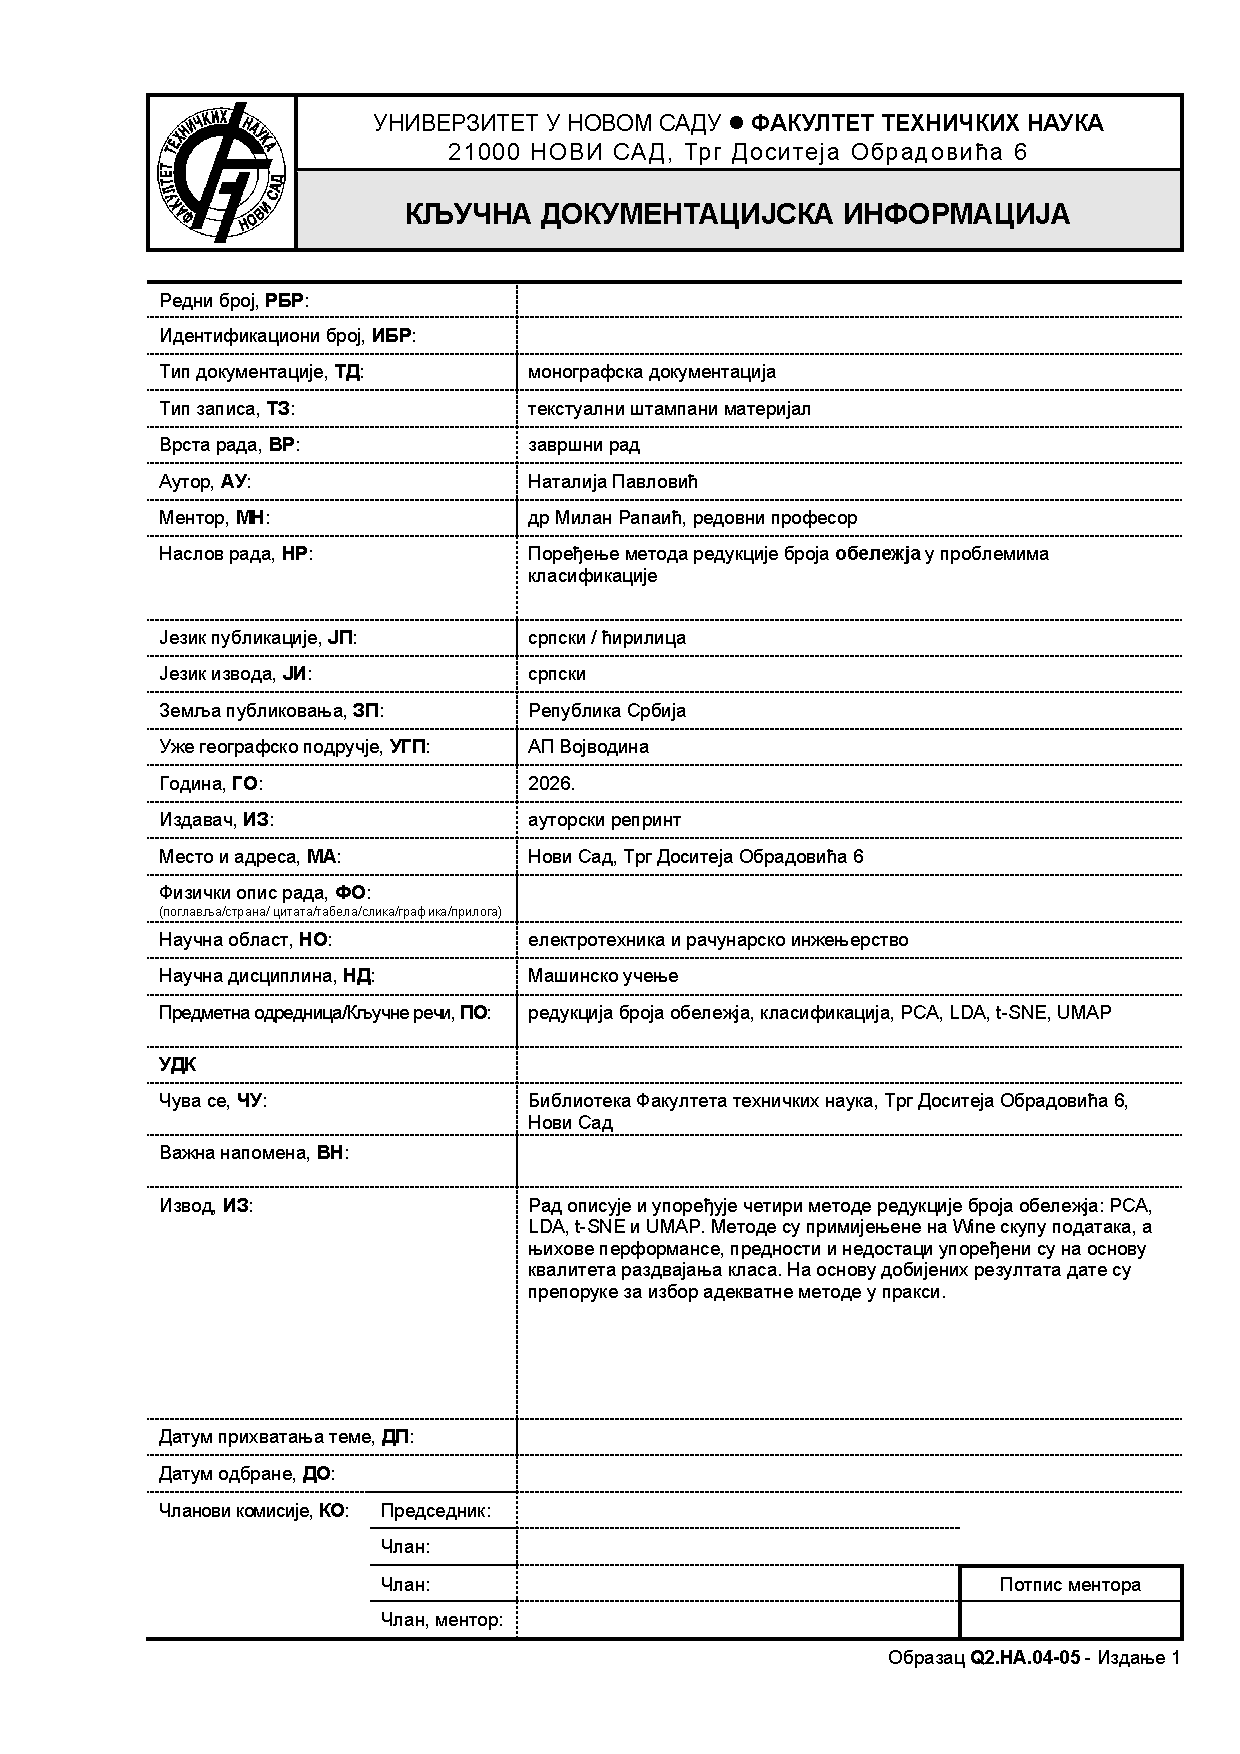
\includepdf[pages=1-2]{DrugaTreca.pdf}
	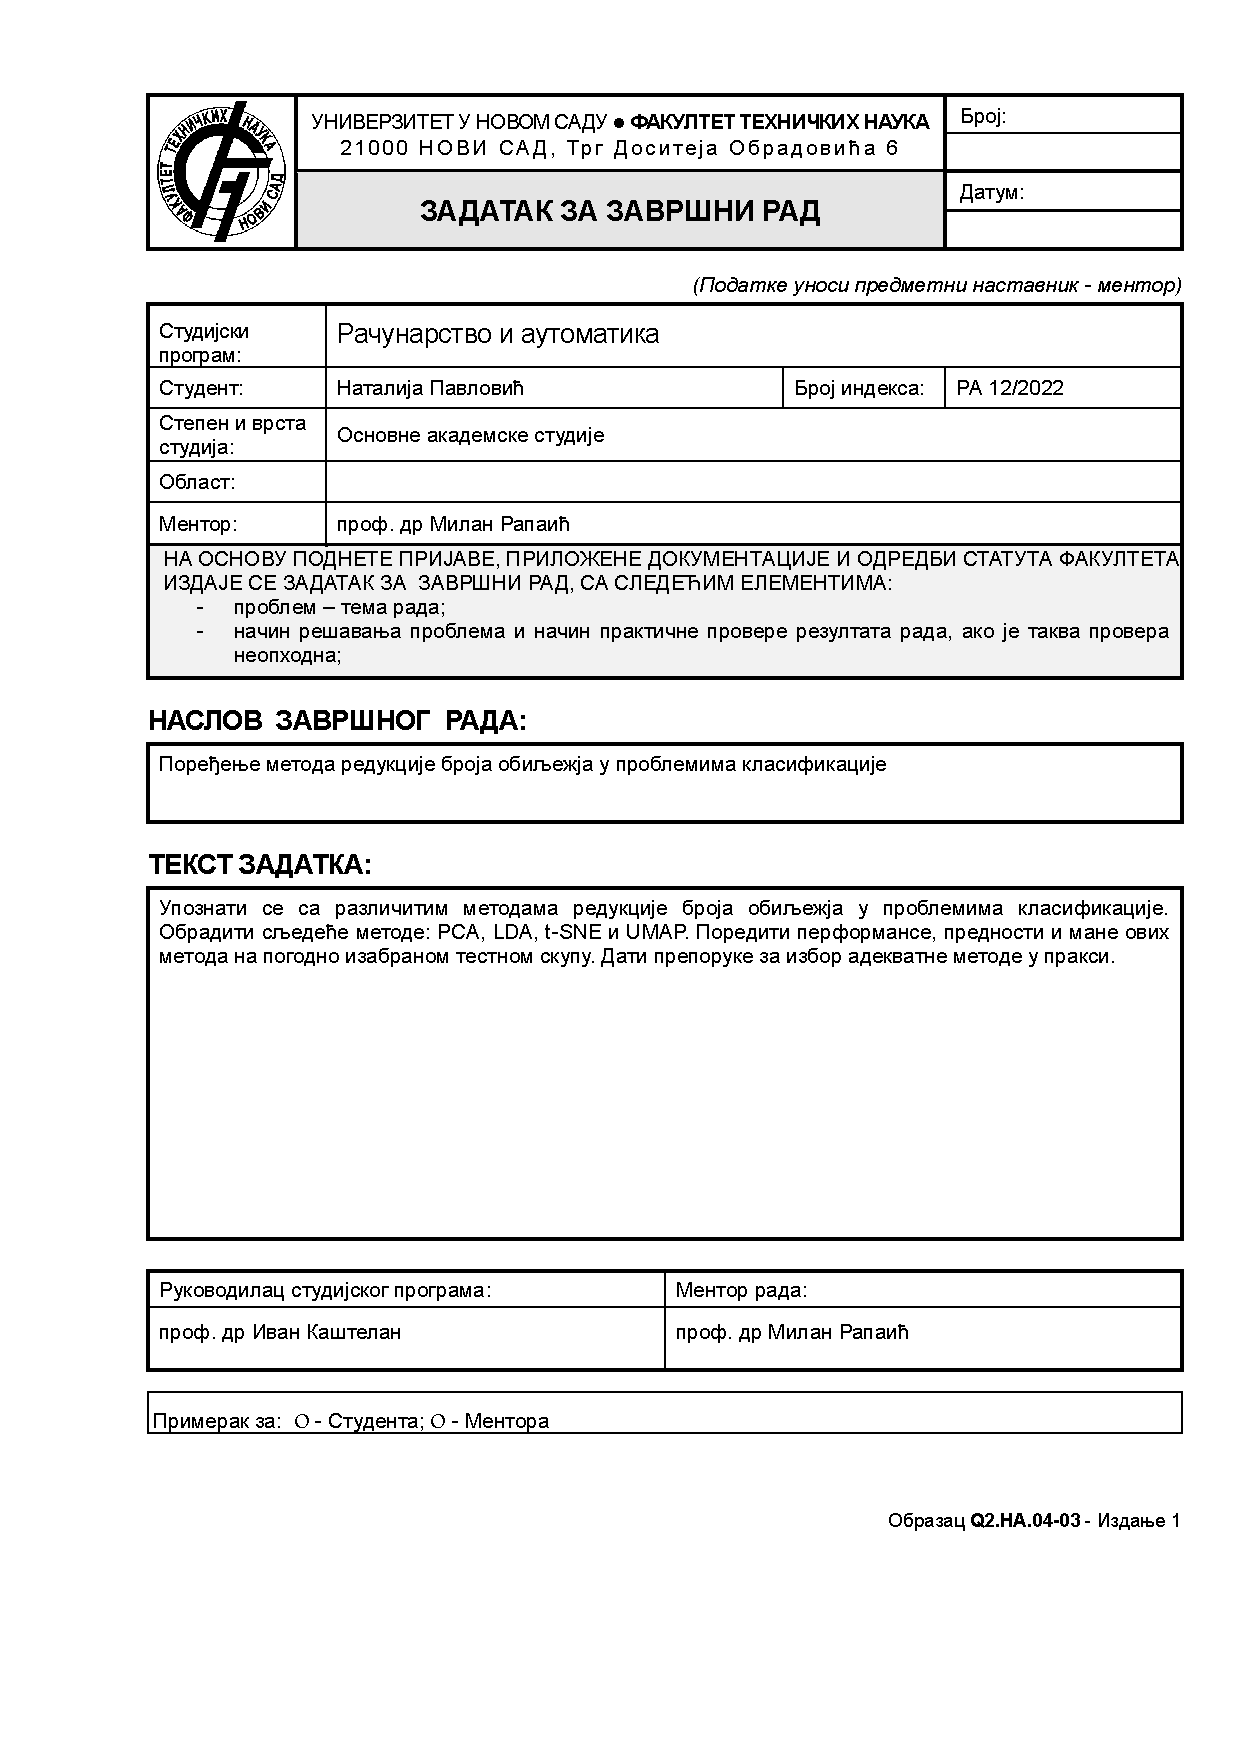
\includepdf[pages=1]{Cetvrta.pdf}
	\tableofcontents
	\afterpage{\blankpage}
	\pagebreak
	
	
	\section{Увод}
	
	У машинском учењу скупови података често садрже велики број карактеристика (енгл. \textit{feature}), у већини случајева стотине или хиљаде. Иако се на први поглед чини да више информација води ка бољим резултатима, у пракси висока димензионалност доноси специфичне изазове који отежавају, а у неким случајевима и онемогућавају директну примjену класичних алгоритама. Овај феномен је познат као проклетство димензионалности (енгл. \textit{curse of dimensionality}). Огледа се у наглом порасту рачунске сложености и повећаној потрошњи меморије што додатно отежава учење и генерализацију модела. Управо због тога, смањење димензионалности (енгл. \textit{dimensionality reduction}) - поступак трансформације података из простора виших димензија у простор нижих димензија, уз задржавање што већег броја корисних информација - представља једну од кључних техника у обради података.
	
	Поред уштеде рачунарских ресурса, смањење димензионалности доноси и друге предности. Уклањањем сувишних и међусобно зависних карактеристика смањује се ризик од преприлагођавања (енгл. \textit{overfitting}), убрзава се тренирање модела, а добијени подаци постају погоднији за визуелизацију, која је у простору високе димензионалности практично немогућа. С друге стране, сваки поступак редукције подразумијева одређени губитак информација, па избор одговарајуће методе зависи од природе података и циља анализе. Управо ова равнотежа између уштеде и очувања информација чини проблем смањења димензионалности темом бројних научних радова.
	
	У овом раду анализираће се четири методе смањења димензионалности: анализа главних компоненти (енгл. \textit{Principal Component Analysis - PCA}), линеарна дискриминантна анализа (енгл. \textit{Linear Discriminant	Analysis - LDA}), стохастичко уметање сусједних тачака са $t$-расподјелом (енгл. \textit{$t$-distributed Stochastic Neighbor Embedding - t-SNE}) и уједначена апроксимација многострукости и пројекција (енгл. \textit{Uniform Manifold Approximation and Projection - UMAP}). Свака од ових метода приступа проблему редукције из другог угла, са различитим претпоставкама, предностима и ограничењима, те ће посебна пажња бити посвећена њиховом међусобном поређењу на истим подацима.
	
	У другом поглављу описан је Wine скуп података који је коришћен у свим експериментима. Треће поглавље покрива линеарне методе, PCA и LDA, са детаљним математичким описом принципа на којима почивају. Четврто поглавље посвећено је нелинеарним методама, t-SNE и UMAP, код којих је нагласак на очувању локалне структуре података. Коначно, пето поглавље садржи нумеричке резултате и поређење свих метода примијењених на истим скупом података, чиме се сагледавају њихове предности и ограничења у пракси.
	
	
	\subsection{Проклетство димензионалности}
	
	Са порастом броја димензија подаци постају све рјеђе распоређени у простору. Ова појава се најлакше може разумјети на једноставном примјеру. Посматрајмо 100 тачака које су насумично изабране из униформне расподјеле на интервалу $(0,1)$. Ако тај интервал подијелимо на десет једнаких дјелова, у сваком дијелу ће се највјероватније наћи по неколико тачака. Ако задржимо исти број тачака, али их сада распоредимо у јединични квадрат, чиме прелазимо на двије димензије, и задржимо исту подјелу простора од $0{,}1$, добијамо 100 ћелија, па је вјероватно да ће неке остати празне. За исте 100 тачака у три димензије број ћелија расте на 1000, тако да ће већина ћелија бити празна. Дакле, како димензија расте, тачке се све више „губе'' у простору.
	
	Ова појава, у којој подаци у високим димензијама увијек изгледају рјетко распоређено без обзира на њихов број, назива се проклетство димензионалности (енгл. \textit{curse of dimensionality}) \cite{bishop2006}. Она представља проблем за велики број алгоритама, јер њихов резултат често зависи од удаљености или густине тачака. Алгоритми засновани на удаљености, као што су $k$ најближих сусједа ($k$-NN), $k$-средина ($k$-Means), губе моћ разликовања, зато што у високим димензијама све тачке постају приближно подједнако удаљене. Модели због великог броја карактеристика лакше упадају у преприлагођавање (енгл. \textit{overfitting}), а тренирање и предвиђање постају спорији. Такође, визуелизација података није могућа без претходне редукције димензионалности.
	
	Један од начина да се овај проблем ријеши јесте пројектовање тачака у простор мање димензије. Идеја је да подаци заправо леже у простору мање димензије, па се њиховом редукцијом губи само мали дио информација, а у неким случајевима овим приступом се уклањају и одударајући подаци. Утицај броја димензија на тачност модела приказан је на слици \ref{fig:curse}. Са слике се види да тачност на оригиналних 100 карактеристика, од којих је само 5 информативно, знатно заостаје за тачношћу која је добијена након примјене PCA или LDA редукције. Из овог примјера можемо да видимо да већи број димензија не значи и бољи резултат.
	
	\begin{figure}[H]
		\centering
		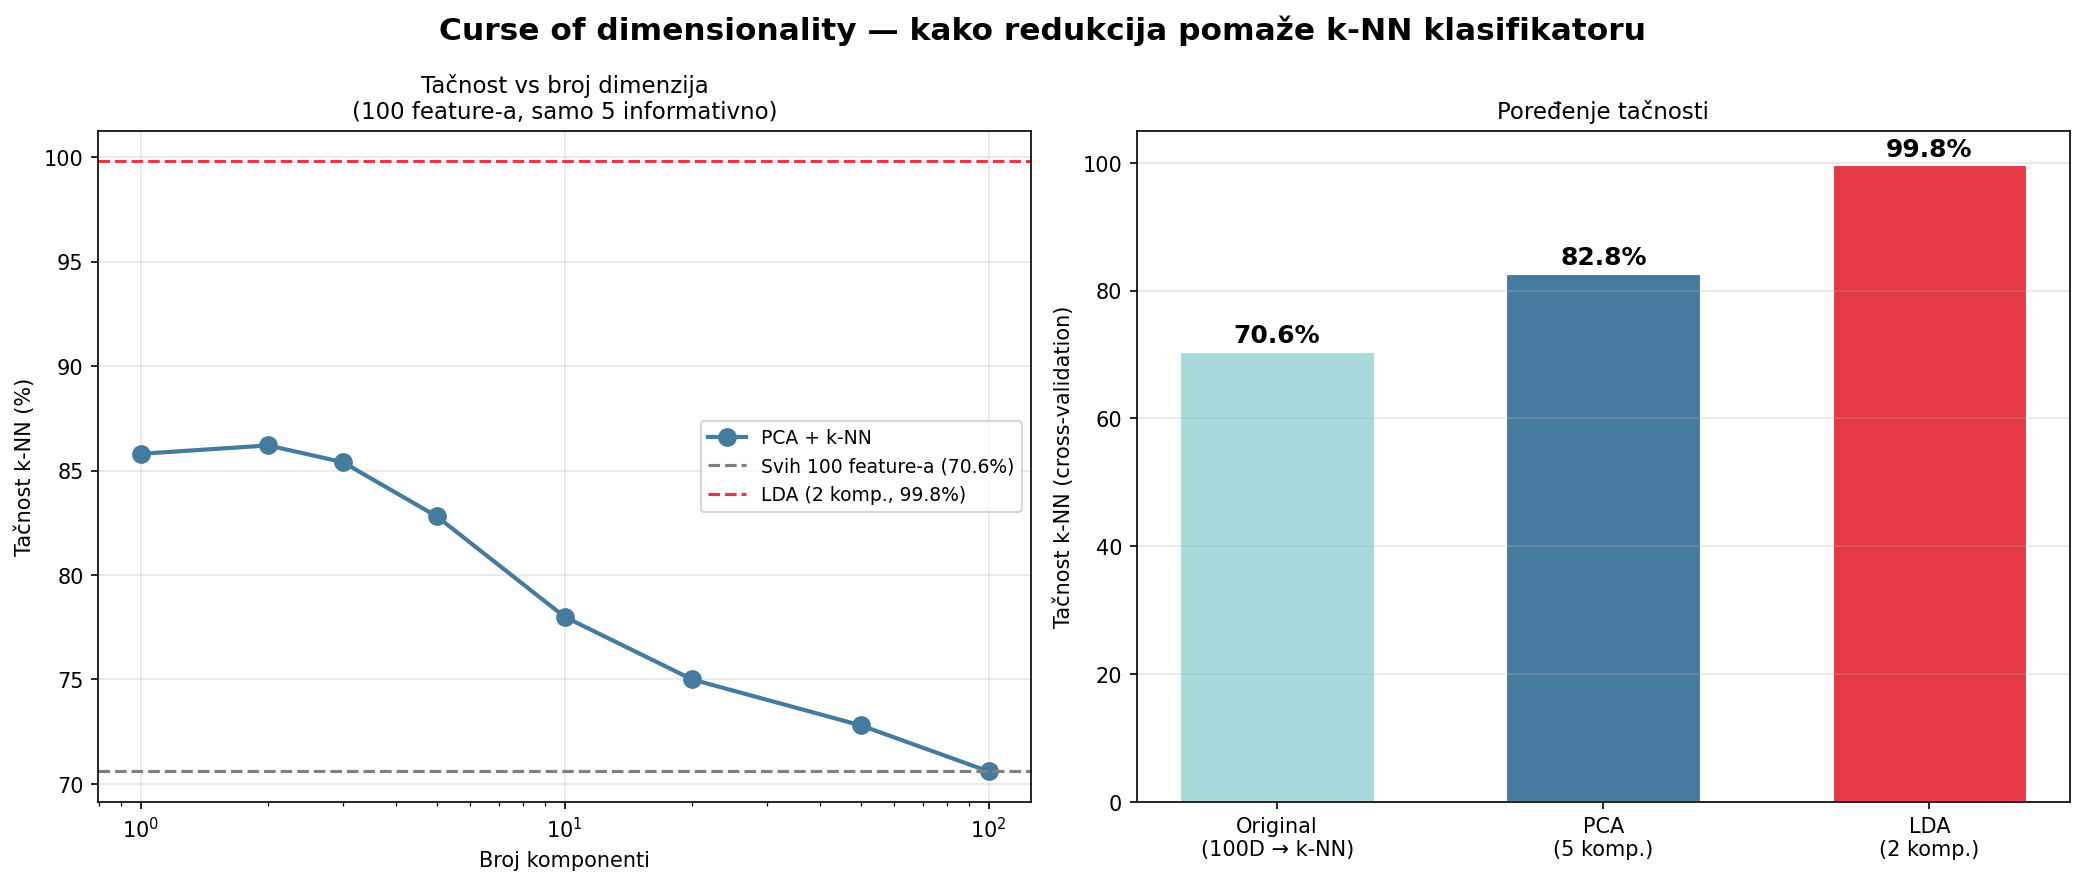
\includegraphics[width=\textwidth]{07_curse_of_dim.png}
		\caption{Проклетство димензионалности - тачност $k$-NN класификатора у зависности од броја димензија и поређење тачности за три приступа.}
		\label{fig:curse}
	\end{figure}
	
	
	\subsection{Зашто смањивати димензије?}
	
	Смањење димензионалности је корисно из неколико разлога:
	\begin{itemize}
		\item убрзава тренирање и смањује меморијске захтјеве;
		\item уклања шум и редундантне карактеристике;
		\item омогућава визуелизацију података пројекцијом на 2Д или 3Д;
		\item побољшава генерализацију модела;
		\item олакшава интерпретацију, односно разумијевање које су карактеристике важне.
	\end{itemize}
	
	
	\subsection{Подела метода}
	
	Методе смањења димензионалности дијеле се према два критеријума.
	
	\textbf{Линеарност:} линеарне (PCA, LDA) наспрам нелинеарних (t-SNE, UMAP). Линеарне методе претпостављају да се подаци могу добро описати линеарним комбинацијама оригиналних карактеристика. Док нелинеарне методе посједују могућност хватања сложенијих, закривљених структура у подацима.
	
	\textbf{Надзор:} ненадгледане (PCA, t-SNE, UMAP) наспрам надгледаних (LDA). Ненадгледане методе користе само улазне податке $\mathbf{X}$ и траже структуру без познавања ознака класа. Док надгледане методе (LDA) користе и ознаке класа $\mathbf{y}$ како би осигурале максималну сепарабилност између њих.
	
	\newpage
	
	
	\section{Скуп података - Вино}
	
	Сви експерименти у овом раду користе Wine скуп података из UCI репозиторијума за машинско учење \cite{wine_dataset}. Скуп садржи резултате хемијске анализе 178 узорака вина из три регије Италије. Циљ је класификовати вино у једну од три класе (сорте) на основу 13 хемијских карактеристика.
	
	Скуп садржи сљедеће карактеристике:
	\begin{itemize}
		\item \textbf{178 узорака} (вина)
		\item \textbf{13 нумеричких карактеристика}: садржај алкохола, јабучна киселина, пепео, алкалност пепела, магнезијум, укупни феноли, флавоноиди, нефлавоноиди, проантоцијани, интензитет боје, нијанса, OD280/OD315, пролин
		\item \textbf{3 класе} (сорте вина): Бароло, Гриньолино, Барбера
	\end{itemize}
	
	Подаци су стандардизовани (средња вриједност 0, стандардна девијација 1) прије примјене алгоритама. Стандардизација је обавезна за PCA и t-SNE јер су ови алгоритми осјетљиви на скалу карактеристика. Без стандардизације, карактеристике са већим опсегом вриједности (нпр. пролин: 278-1680) би доминирале резултатом у односу на карактеристике са мањим опсегом (нпр. нијанса: 0.48-1.71).
	
	\newpage
		
	
	\section{Линеарне методе смањења димензионалности}
	
	
	\subsection{PCA - Анализа главних компоненти}
	
	Анализа главних компоненти (енгл. \textit{Principal Component Analysis}, PCA) једна је од најпознатијих и најшире коришћених метода линеарне редукције димензионалности \cite{bishop2006, shlens2014}. Ријеч је о \textbf{ненадгледаној} методи, што значи да не користи податке о класама, нити су јој они потребни - она посматра искључиво саме податке и тражи правце дуж којих се они највише разликују, односно правце највеће варијансе. Управо ти правци, поређани од оног са највећом ка оном са најмањом варијансом, представљају главне компоненте.
	
	Циљ методе је да пронађе нови координатни систем чије су осе, главне компоненте, поређане према количини варијансе коју објашњавају. Прва главна компонента (PC1) објашњава највећи дио варијансе у подацима, друга (PC2) сљедећи по величини, и тако редом. Пошто прве компоненте носе највећи дио информација, задржавањем само неколико њих добија се \textbf{нискодимензионална репрезентација} која чува главне особине полазног скупа, док се преостале компоненте, које углавном садрже шум и ситне варијације, одбацују.
	
	При оваквој редукцији један дио информација се неминовно губи, али је тај губитак мали и контролисан - задржава се онолико компоненти колико је потребно да се сачува жељени проценат варијансе (најчешће око 95\%). Треба нагласити да PCA није намијењена раздвајању класа: пошто не познаје ознаке класа, она чува варијансу, а не сепарабилност. Ипак, ако се узорци исте класе у оригиналном простору природно групишу, ти кластери често остају уочљиви и у пројекцији, што PCA чини корисном и за визуелно откривање структуре у подацима.
	
	
	\subsubsection{Поступак}
	
	PCA се изводи у сљедећим корацима \cite{matf_pca}.
	
	\textbf{Корак 1 - Стандардизација података.} Најприје се свака карактеристика центрира, тако што се од ње одузме њена средња вриједност, а затим скалира дијељењем са стандардном девијацијом:
	\begin{equation} \label{eq:pca_std}
	\mathbf{X}_{std} = \frac{\mathbf{X} - \mu}{\sigma}
	\end{equation}
	Овдје је $\mathbf{X}$ матрица података димензија $n \times d$, у којој сваки од $n$ редова представља један узорак, а свака од $d$ колона једну карактеристику:
	\begin{equation} \label{eq:pca_matrix}
		\mathbf{X} =
		\begin{bmatrix}
			x_{11} & x_{12} & \cdots & x_{1d} \\
			x_{21} & x_{22} & \cdots & x_{2d} \\
			\vdots & \vdots & \ddots & \vdots \\
			x_{n1} & x_{n2} & \cdots & x_{nd}
		\end{bmatrix},
	\end{equation}
	гдје елемент $x_{ij}$ означава вриједност $j$-те карактеристике за $i$-ти узорак. Вектори $\boldsymbol{\mu}$ и $\boldsymbol{\sigma}$ садрже средње вриједности и стандардне девијације свих $d$ карактеристика, па се одузимање и дијељење у формули врше по колонама.
	
	Средња вриједност $\mu_j$ сваке карактеристике рачуна се као аритметичка средина њених вриједности по свим узорцима:
	\begin{equation} \label{eq:pca_mean}
		\mu_j = \frac{1}{n} \sum_{i=1}^{n} x_{ij},
	\end{equation}
	а одговарајућа стандардна девијација $\sigma_j$ као:
	\begin{equation} \label{eq:pca_std_dev}
		\sigma_j = \sqrt{\frac{1}{n} \sum_{i=1}^{n} (x_{ij} - \mu_j)^2}.
	\end{equation}
	Овим кораком све карактеристике се доводе на исту скалу и постају међусобно упоредиве.
	
	\textbf{Корак 2 - Матрица коваријанси.} Након што су подаци стандардизовани, рачуна се матрица коваријанси $\mathbf{C}$ димензија $d \times d$, гдје $d$ означава број карактеристика (за Wine скуп $d = 13$). Ова матрица описује како се карактеристике међусобно понашају: њен елемент $C_{ij}$ говори колико се вриједности карактеристика $i$ и $j$ мијењају заједно. Позитивна вриједност значи да оне расту заједно, негативна да једна расте док друга опада, а вриједност близу нуле да међу њима нема изражене везе. Матрица коваријанси се рачуна као
	\begin{equation} \label{eq:pca_cov}
		\mathbf{C} = \frac{1}{n-1}\,\mathbf{X}_{std}^T \mathbf{X}_{std},
	\end{equation}
	гдје је $n$ број узорака, а $\mathbf{X}_{std}$ стандардизована матрица података из претходног корака.
	
	\textbf{Корак 3 - Сопствене вриједности и вектори.} За добијену матрицу коваријанси рјешава се проблем сопствених вриједности - задатак у коме се траже посебни правци које матрица $\mathbf{C}$ не мијења, већ их само развлачи или скупља. Он се записује као:
	\begin{equation} \label{eq:pca_eig}
		\mathbf{C}\,\mathbf{v} = \lambda\,\mathbf{v},
	\end{equation}
	гдје је $\mathbf{v}$ сопствени вектор (енгл. \textit{eigenvector}), а $\lambda$ припадајућа сопствена вриједност (енгл. \textit{eigenvalue}). Сваки сопствени вектор одређује правац једне главне компоненте, док одговарајућа сопствена вриједност говори колику варијансу подаци имају дуж тог правца.
	
	\textbf{Корак 4 - Сортирање и одабир компоненти.} Пошто свака сопствена вриједност говори колику варијансу носи њен правац, сопствени вектори се распореде по величини сопствених вриједности, од највеће ка најмањој. На тај начин се на почетку налазе они правци дуж којих се подаци највише разликују, односно они који носе највише информација. Затим се бира првих $k$ сопствених вектора, који заједно објашњавају довољан дио укупне варијансе, најчешће око 95\%. Тих $k$ изабраних вектора постављају се као колоне матрице пројекције $\mathbf{W}$:
	\begin{equation} \label{eq:pca_W_select}
		\mathbf{W} = [\,\mathbf{v}_1 \;\; \mathbf{v}_2 \;\; \cdots \;\; \mathbf{v}_k\,],
	\end{equation}
	гдје су $\mathbf{v}_1, \mathbf{v}_2, \dots, \mathbf{v}_k$ сопствени вектори са $k$ највећих сопствених вриједности. Управо избор броја $k$ одређује колико ће димензија имати редуковани простор.
	
	\textbf{Корак 5 - Пројекција.} На крају се подаци пребацују у нови простор мање димензије. Свака тачка (узорак) множи се матрицом $\mathbf{W}$ и тако умјесто $d$ оригиналних вриједности добија $k$ нових координата:
	\begin{equation} \label{eq:pca_proj}
		\mathbf{Z} = \mathbf{X}_{std}\,\mathbf{W}.
	\end{equation}
	Резултат је матрица $\mathbf{Z}$, у којој сваки ред одговара једном узорку, али сада описаном помоћу само $k$ главних компоненти. Другим ријечима, полазна матрица димензија $n \times d$ своди се на матрицу димензија $n \times k$. За Wine скуп то значи да се $178 \times 13$ (178 узорака, 13 карактеристика) своди на $178 \times 2$ - сваки узорак је сада приказан помоћу само двије вриједности. 
	Са овим кораком завршава се поступак PCA алгоритма и добија се коначни, редуковани приказ података у простору мање димензије.
	
	
	\subsubsection{Матрице у PCA}
	
	Кроз цио поступак PCA појављују се четири важне матрице. Овдје је укратко објашњено шта свака од тих матрица представља.
	
	\textbf{$\mathbf{X}$ - Матрица података} (димензије $n \times d$, тј. $178 \times 13$ за Wine скуп). У њој се налазе полазни подаци: сваки ред је један узорак (једно вино), а свака колона једна карактеристика. Након стандардизације свака колона има средњу вриједност 0 и стандардну девијацију 1.
	
	\textbf{$\mathbf{C}$ - Матрица коваријанси} (димензије $d \times d$, тј. $13 \times 13$). Показује како се карактеристике међусобно понашају, односно колико се сваки пар карактеристика мијења заједно. А њени дијагонални елементи $C_{ii}$ представљају варијансе појединачних карактеристика.
	
	\textbf{$\mathbf{W}$ - Матрица пројекције} (димензије $d \times k$, тј. $13 \times 2$ за редукцију на двије димензије). Њене колоне су одабрани сопствени вектори матрице $\mathbf{C}$, распоређени од оног са највећом ка оном са најмањом сопственом вриједношћу. Помоћу ове матрице подаци се пребацују у нови простор мање димензије.
	
	\textbf{$\mathbf{Z}$ - Матрица пројицираних података} (димензије $n \times k$, тј. $178 \times 2$). Представља крајњи резултат PCA. У њој је сваки узорак приказан помоћу свега $k$ нових вриједности умјесто првобитних $d$.
	
	
	\subsubsection{Scree plot и објашњена варијанса}
	
	\textit{Scree plot} је график који показује колико варијансе носи свака компонента. Помаже да се одлучи колико компоненти је неопходно задржати да би се очувао задати проценат варијансе. На Wine скупу прва компонента објашњава око 36\% укупне варијансе, а друга око 19\%, па заједно носе приближно 55\% свих информација. То значи да пројекцијом са 13 на 2 димензије губимо око 45\% информација, али добијамо могућност да податке прикажемо на графику. Ако желимо да сачувамо више информација, потребно је задржати више компоненти - да бисмо прешли праг од 95\% укупне варијансе, потребно је да се сачува око 10 компоненти.
	
	\begin{figure}[h!]
		\centering
		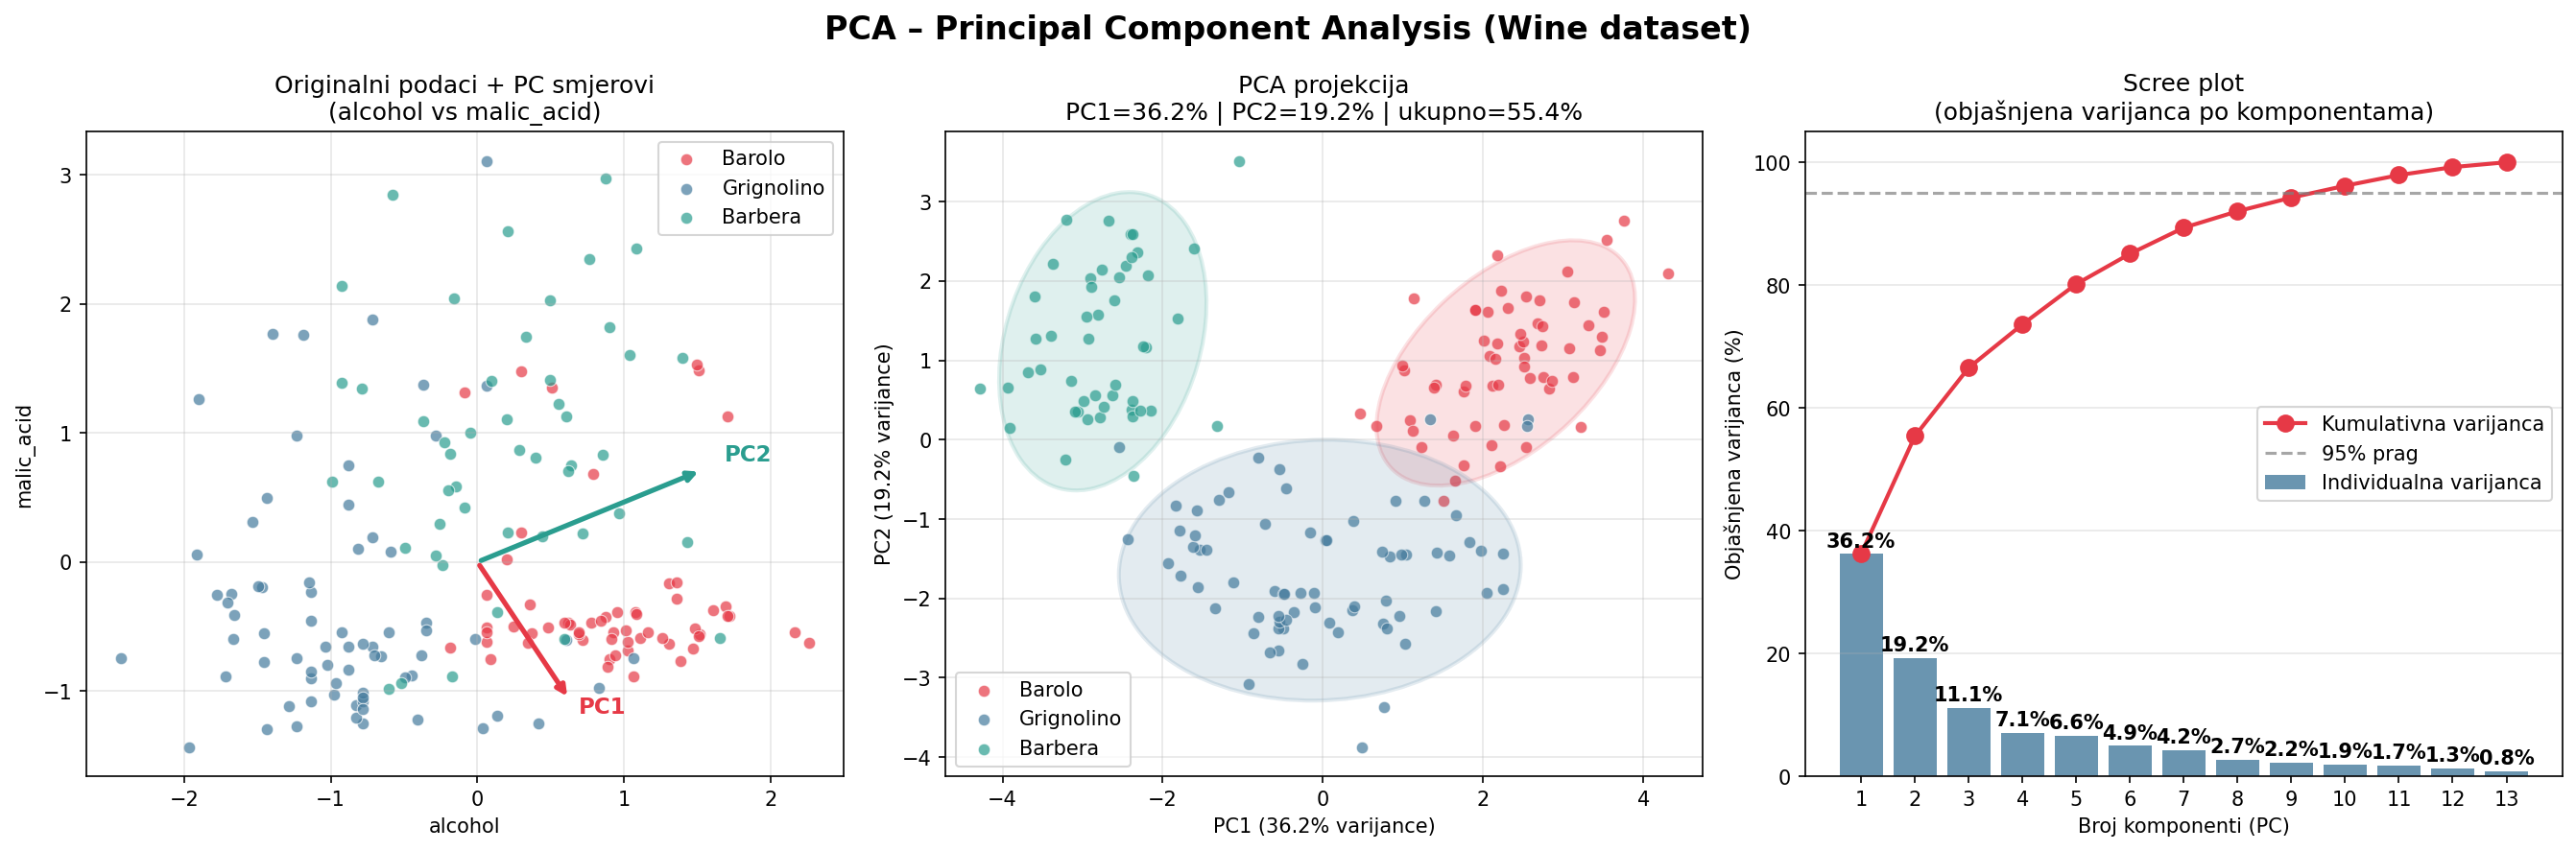
\includegraphics[width=\textwidth]{01_pca_wine.png}
		\caption{PCA на Wine скупу: оригинални подаци са PC правцима (лијево), PCA пројекција у 2Д са елипсама поузданости (средина) и \textit{scree plot} - објашњена варијанса по компонентама (десно).}
		\label{fig:pca_wine}
	\end{figure}
	
	Када Wine скуп пројектујемо на прве двије главне компоненте, добијамо његов приказ у двије димензије (слика \ref{fig:pca_wine}). На њему се виде три групе вина које су дјелимично раздвојене, а око сваке је нацртана елипса која обухвата око 95\% тачака те класе. Групе се ипак донекле преклапају, што је очекивано - PCA није направљена да раздваја класе, већ само да сачува што више варијансе у подацима.
	
	
	\subsubsection{Тежине (\textit{loadings}) - Интерпретација компоненти}
	
	Пошто главне компоненте представљају линеарне комбинације оригиналних карактеристика, оне саме по себи немају очигледно значење - PC1 и PC2 су само нове осе, не представљају нешто што можемо директно измјерити. Да бисмо разумјели шта нека компонента заправо представља, користе се тежине (\textit{loadings}).
	
	Тежине показују колико свака оригинална карактеристика доприноси појединој главној компоненти. Свака компонента добија по један број за сваку карактеристику, број може бити позитиван или негативан. Што је апсолутна вриједност броја већа, то та карактеристика јаче утиче на дату компоненту. Вриједност близу нуле значи да дата карактеристика готово да не доприноси компоненти. Знак вриједности, позитиван или негативан, показује да ли карактеристика дјелује у истом или у супротном смјеру од компоненте.
	
	Управо ту се види зашто су тежине корисне: оне компоненти дају смисао. Умјесто да PC1 остане само апстрактна оса, из вриједности тежина можемо прочитати шта она заправо мјери. Ако, рецимо, феноли и флавоноиди највише доприносе првој компоненти, онда PC1 у суштини описује садржај фенолних једињења у вину.
	
	На слици \ref{fig:pca_loadings} приказана је топлотна мапа (\textit{heatmap}) вриједности тежина, гдје боја сваког поља показује допринос одговарајуће карактеристике одговарајућој компоненти. Тамније боје означавају јак утицај, а свјетлије слаб. Оваква мапа омогућава да се уочи које карактеристике доминирају у којој компоненти.
	
	\begin{figure}[H]
		\centering
		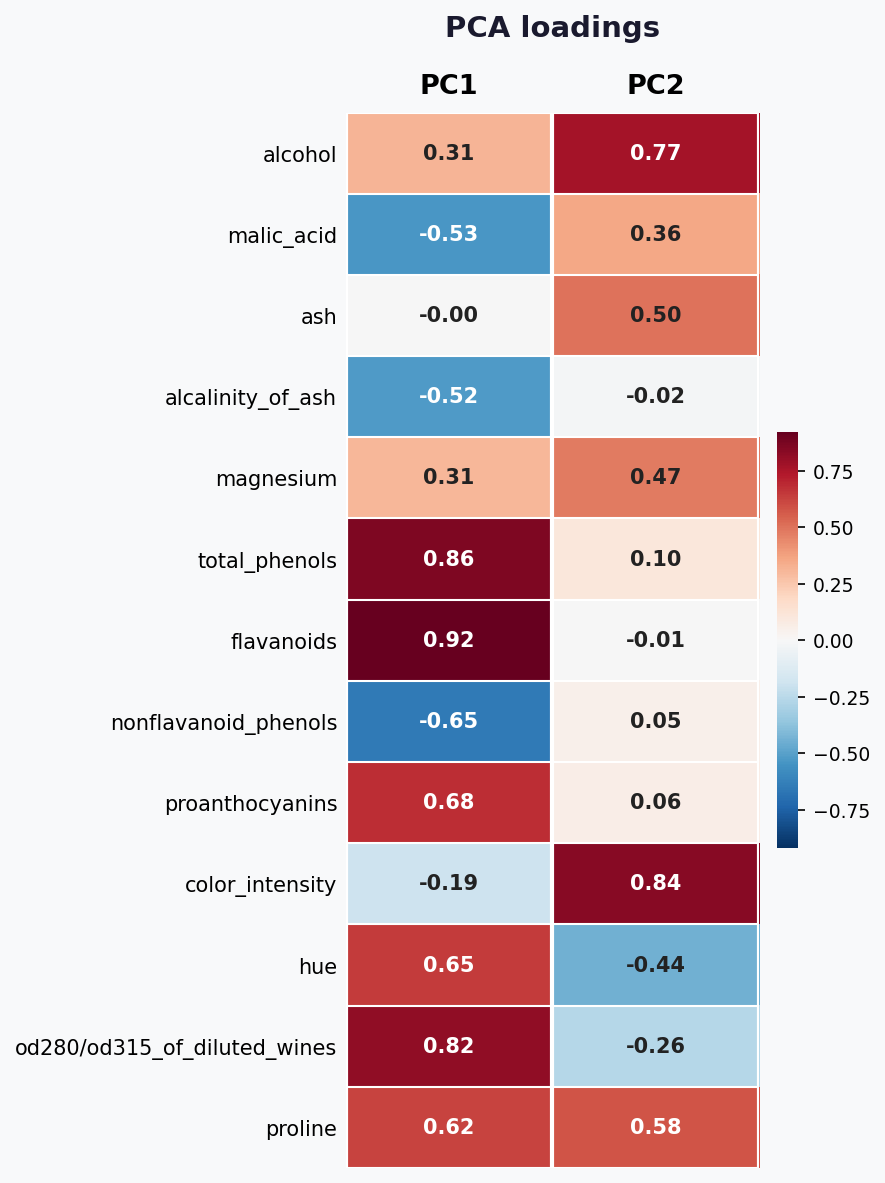
\includegraphics[width=7cm]{06a_pca_loadings.png}
		\caption{Топлотна мапа вриједности тежина за PCA. Вриједности показују допринос сваке карактеристике свакој компоненти.}
		\label{fig:pca_loadings}
	\end{figure}
	
	
	\subsubsection{Ограничења PCA}
	
	PCA полази од претпоставке да су најважнији они правци дуж којих подаци имају највећу варијансу. То, међутим, није увијек тачно. Понекад се разлика између класа налази баш у правцу мале варијансе - у том случају PCA тај правац занемари, а задржи онај који носи више варијансе, али не и корисну информацију о класама. На слици \ref{fig:pca_fail} приказана су два таква случаја у којима PCA заказује.
	
	\textbf{Полумјесеци.} У горњем примјеру подаци двије класе распоређени су у облику два полумјесеца. То је нелинеарна структура коју PCA не умије да ,,исправи'', јер умије само да ротира и пројектује податке праволинијски. Када их сведе на једну димензију, два полумјесеца се преклопе и класе се потпуно измијешају.
	
	\textbf{Варијанса шума већа од варијансе сигнала.} У доњем примјеру су двије класе лијепо раздвојене у једном правцу, али у том правцу је варијанса мала. У другом правцу, гдје нема никакве разлике међу класама, налази се шум - али са већом варијансом. Пошто PCA бира правац по величини варијансе, изабере баш правац шума и тако изгуби информацију која раздваја двије класе.
	
	У оба случаја видимо исту слабост: PCA гледа само колику варијансу неки правац носи, а не и да ли тај правац заиста раздваја класе. Зато PCA није поуздана када је циљ раздвајање класа, за то су погоднији надгледани приступи попут LDA, о којој ће бити ријечи у наставку.
	
	\begin{figure}[H]
		\centering
		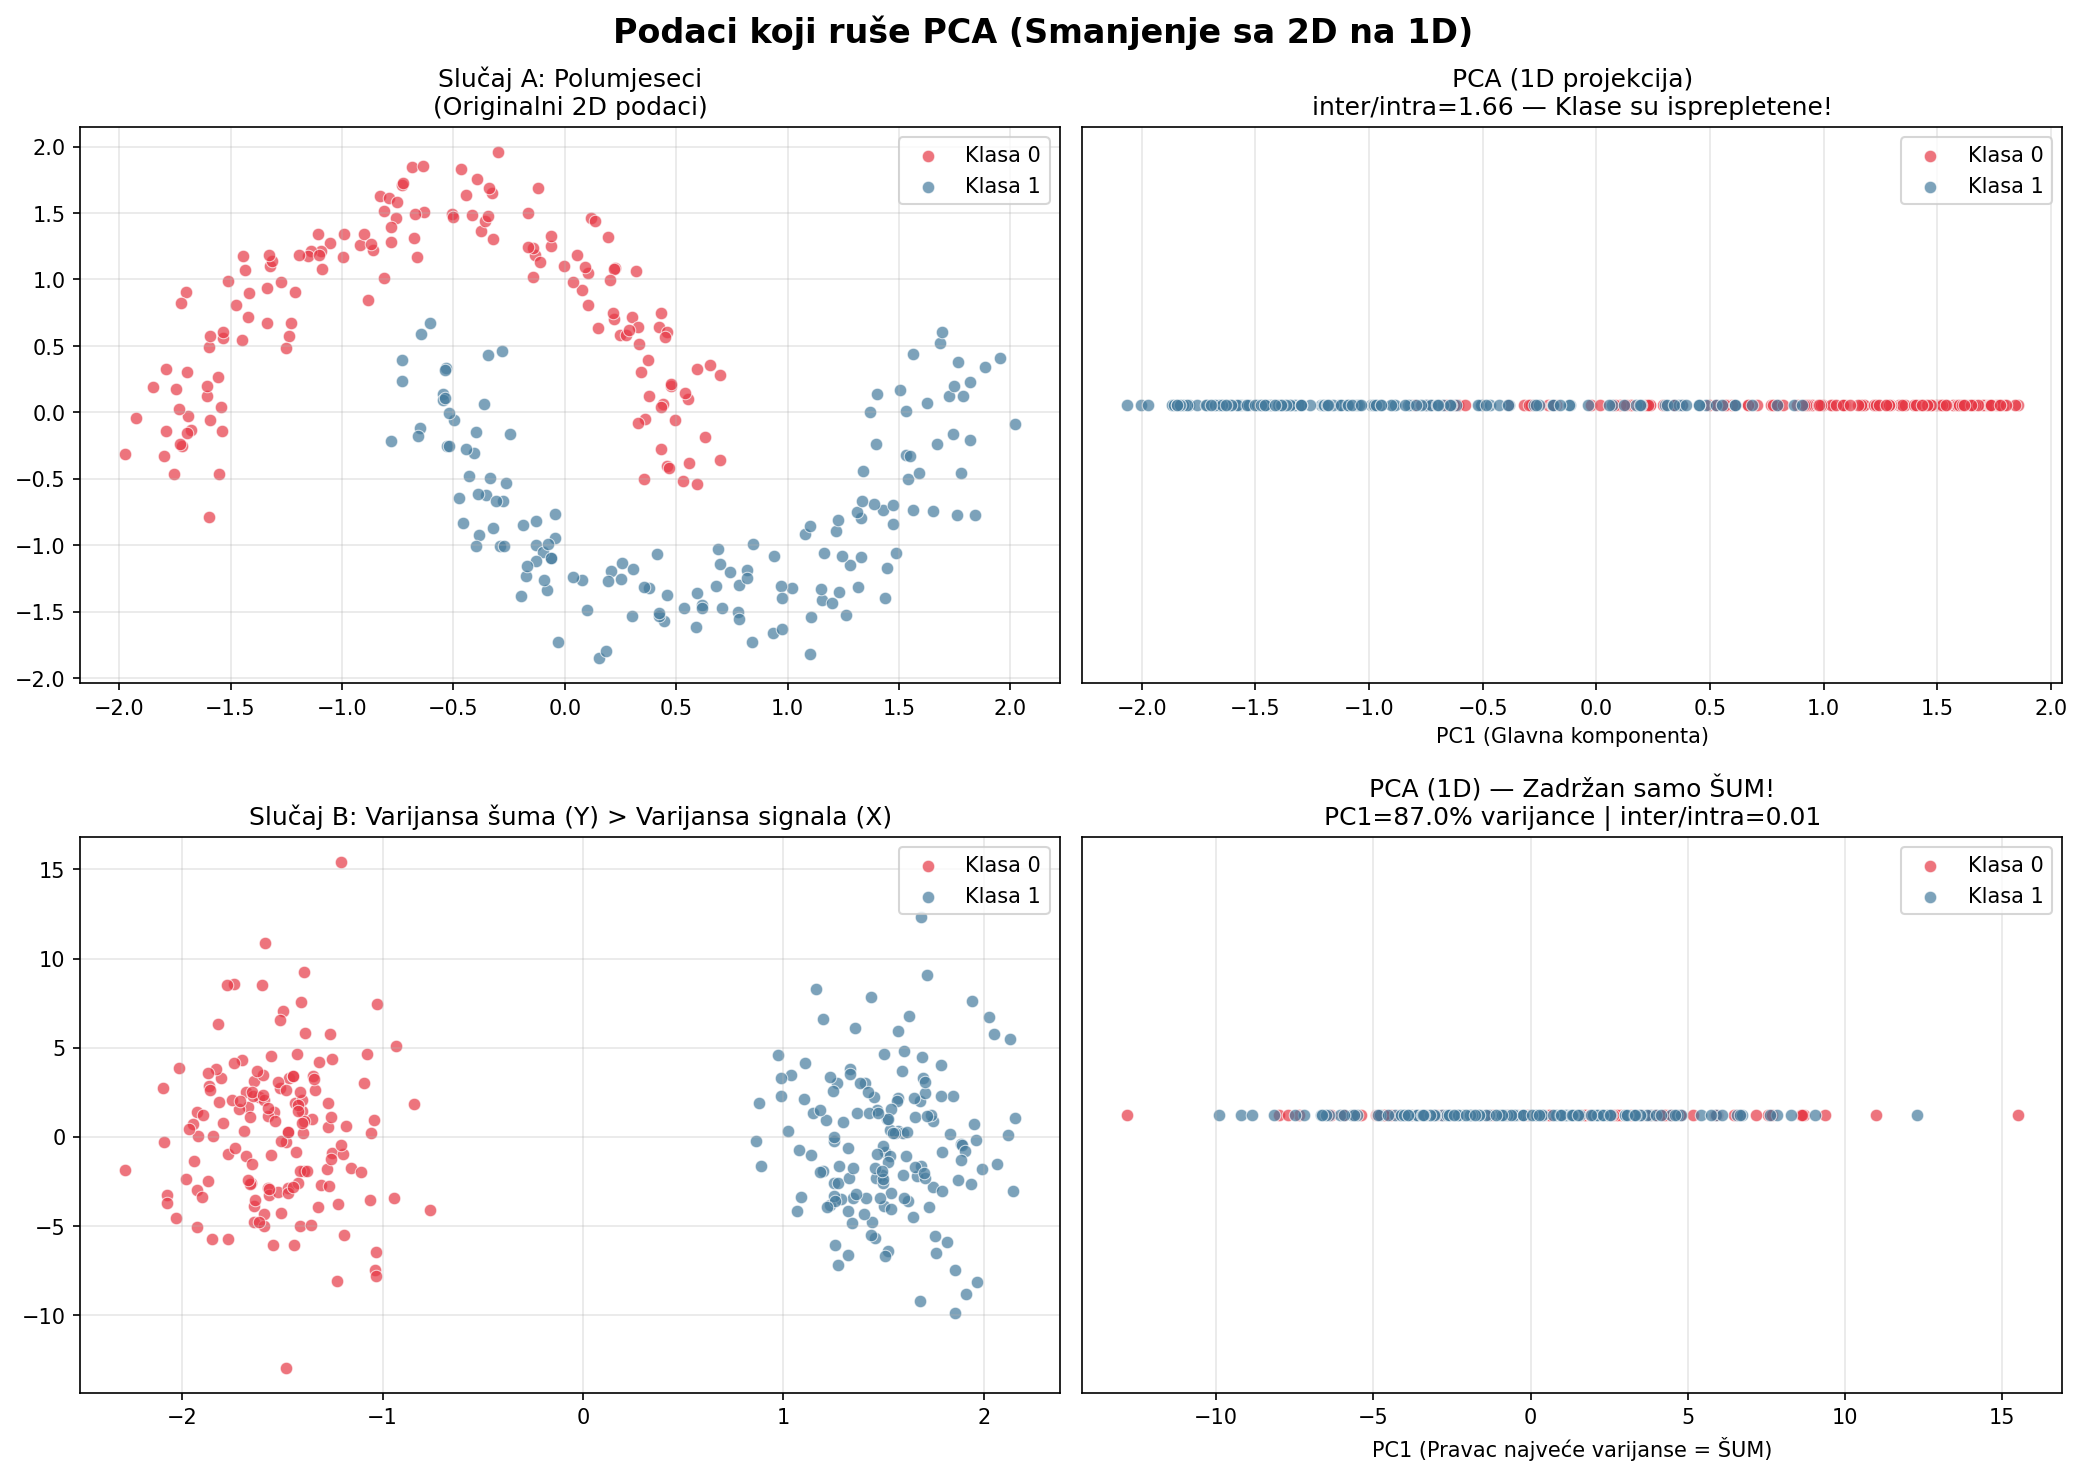
\includegraphics[width=\textwidth]{03_pca_failures.png}
		\caption{Случајеви гдје PCA заказује: полумјесеци (нелинеарна структура, горе) и подаци гдје шум има већу варијансу од сигнала (доле). У оба случаја PCA преклапа класе.}
		\label{fig:pca_fail}
	\end{figure}
	
	\clearpage
	
	
	\subsection{LDA - Линеарна дискриминантна анализа}
	
	Линеарна дискриминантна анализа (енгл. \textit{Linear Discriminant Analysis}, LDA) је метода линеарне редукције димензионалности, али са другачијим циљем од PCA. За разлику од PCA, која је ненадгледана и не зна ништа о класама, LDA је \textbf{надгледана} метода која користи ознаке класа, односно податак о томе којој класи сваки узорак припада.
	
	Управо у томе је кључна разлика. PCA тражи правце дуж којих се подаци највише разликују, без обзира на класе, па се може десити да ти правци уопште не раздвајају класе. С друге стране LDA има само један циљ, а то је да пронађе правац дуж кога су класе што боље раздвојене. Да би то постигла, LDA истовремено гледа двије ствари. Прво, тежи да центри различитих класа буду што удаљенији један од другог, како би се класе што мање преклапале. Друго, тежи да тачке унутар исте класе буду што ближе једна другој, односно да свака класа буде што компактнија.
	
	Другим ријечима, LDA максимизује однос расипања \textit{између} класа и расипања \textit{унутар} класа. Пројекција коју на крају добијемо распоређује податке тако да су класе јасно одвојене, а тачке исте класе груписане на једном мјесту. Због тога LDA даје боље раздвојене класе од PCA, али уз ограничење: методи су потребни подаци о класама, односно може се примијенити само када су ознаке класа унапријед познате.
	
	
	\subsubsection{Фишеров критеријум сепарабилности}
	
	Да би пронашла најбољи правац за раздвајање класа, LDA користи Фишеров критеријум, ознаке $J$. То је мјера која говори колико су класе добро раздвојене дуж неког правца $\mathbf{w}$. LDA тражи баш онај правац за који је вриједност $J$ највећа:
	\begin{equation} \label{eq:fisher}
		J(\mathbf{w}) = \frac{\mathbf{w}^T \mathbf{S}_B\, \mathbf{w}}{\mathbf{w}^T \mathbf{S}_W\, \mathbf{w}},
	\end{equation}
	гдје је $\mathbf{S}_B$ матрица расипања између класа (енгл. \textit{between-class scatter}), а $\mathbf{S}_W$ матрица расипања унутар класа (енгл. \textit{within-class scatter}).
	
	Идеја иза овог разломка је једноставна. У бројиоцу се налази расипање између класа - што су центри класа удаљенији један од другог, то је ова вриједност већа. У имениоцу је расипање унутар класа - што су тачке исте класе ближе једна другој, то је ова вриједност мања. Пошто LDA жели да класе буду што удаљеније, а истовремено што компактније, тражи правац за који је бројилац велик, а именилац мали. Тада је и цио разломак, односно вриједност $J$, највећи. Укратко, велико $J$ значи да су класе међусобно добро раздвојене, а тачке унутар сваке класе збијене на једном мјесту.
	
	
	\subsubsection{Поступак}
	
	\textbf{Корак 1 - Средње вриједности класа.} Најприје се за сваку класу $c$ рачуна њена средња вриједност $\boldsymbol{\mu}_c$, тако што се узме просјек свих узорака који припадају тој класи. Та вриједност се назива центроид и представља ,,средиште'' класе, односно тачку око које су распоређени њени узорци. Поред тога, рачуна се и укупна средња вриједност $\boldsymbol{\mu}$ свих података, без обзира на класу, која представља средиште цијелог скупа. Ове средње вриједности су основа за наредне кораке: помоћу њих ће се мјерити колико су класе међусобно удаљене и колико су њихови узорци распршени.
	
	\textbf{Корак 2 - Матрица расипања унутар класа $\mathbf{S}_W$.} Ова матрица нам говори колико су узорци унутар исте класе распршени, то јест колико су ,,разбацани'' око центра своје класе. Замислимо да свака класа има своје средиште (центроид $\boldsymbol{\mu}_c$), а око њега су распоређени сви узорци те класе. За сваки узорак гледамо колико је удаљен од тог средишта, и све те удаљености саберемо - прво унутар једне класе, а затим и за све класе заједно:
	\begin{equation} \label{eq:sw}
		\mathbf{S}_W = \sum_c \sum_{\mathbf{x} \in \text{класа}_c} (\mathbf{x} - \boldsymbol{\mu}_c)(\mathbf{x} - \boldsymbol{\mu}_c)^T.
	\end{equation}
	Ако су узорци исте класе збијени близу свог центроида, ова вриједност је мала и кажемо да је класа компактна. Ако су разбацани, вриједност је велика. Пошто LDA жели да свака класа буде што збијенија, тежи да $\mathbf{S}_W$ буде што мања.
	
	\textbf{Корак 3 - Матрица расипања између класа $\mathbf{S}_B$.} Док претходна матрица гледа шта се дешава \textit{унутар} класа, ова гледа однос \textit{између} класа - колико су средишта различитих класа међусобно удаљена. Сада замислимо да поред средишта сваке класе постоји и једно заједничко средиште свих података ($\boldsymbol{\mu}$). За сваку класу гледамо колико је њен центар удаљен од тог заједничког центра:
	\begin{equation} \label{eq:sb}
		\mathbf{S}_B = \sum_c n_c\,(\boldsymbol{\mu}_c - \boldsymbol{\mu})(\boldsymbol{\mu}_c - \boldsymbol{\mu})^T.
	\end{equation}
	Свака удаљеност се још помножи бројем узорака у тој класи ($n_c$), како би класе са више узорака имале већи утицај. Ако су центри класа далеко један од другог, ова вриједност је велика и класе су добро раздвојене. LDA жели баш то, па тежи да $\mathbf{S}_B$ буде што већа.
	
	\textbf{Корак 4 - Генерализовани проблем сопствених вриједности.} Пошто смо у претходним корацима израчунали обје матрице расипања, сада треба пронаћи правац који истовремено даје велику раздвојеност између класа и малу распршеност унутар класа, то је управо онај правац који максимизује Фишеров критеријум. Тај правац се добија рјешавањем сљедеће једначине:
	\begin{equation} \label{eq:lda_eig}
		\mathbf{S}_W^{-1}\,\mathbf{S}_B\,\mathbf{w} = \lambda\,\mathbf{w}.
	\end{equation}
	Ово је сличан проблем сопствених вриједности као код PCA, само што се овдје не користи матрица коваријанси, већ комбинација двију матрица расипања. Сопствени вектори $\mathbf{w}$ које добијемо представљају тражене правце дуж којих су класе најбоље раздвојене - они се називају дискриминанте. Одговарајућа сопствена вриједност $\lambda$ говори колико је добро раздвајање дуж тог правца: што је $\lambda$ већа, то је раздвојеност класа боља.
	
	\textbf{Корак 5 - Број дискриминанти.} За разлику од PCA, гдје можемо задржати онолико компоненти колико желимо, LDA има ограничење на број дискриминанти. Максималан број дискриминантних оса је $C-1$, гдје је $C$ број класа. Разлог је то што $C$ центара класа увијек лежи у простору димензије $C-1$, па више од толико праваца није ни могуће добити. За Wine скуп, који има 3 класе, то значи да постоје највише 2 дискриминанте, које означавамо са LD1 и LD2.
	
	\textbf{Корак 6 - Пројекција.} На крају се, слично као код PCA, подаци пребацују у нови простор мање димензије. Сваки узорак се помножи матрицом $\mathbf{W}_{LDA}$, чије су колоне изабране дискриминанте, и тако добија нове координате у простору дефинисаном добијеним правцима:
	\begin{equation} \label{eq:lda_proj}
		\mathbf{Z}_{LDA} = \mathbf{X}_{std}\,\mathbf{W}_{LDA}.
	\end{equation}
	Резултат је матрица $\mathbf{Z}_{LDA}$, у којој је сваки узорак приказан помоћу свега неколико вриједности (за Wine скуп двије - LD1 и LD2), али тако да су класе што боље раздвојене.
	
	
	\subsubsection{Матрице у LDA}
	
	Кроз поступак LDA појављује се пет матрица. Овдје је укратко објашњено шта свака од њих представља.
	
	\textbf{$\mathbf{X}$ - Матрица података} (димензије $178 \times 13$). Стандардизована матрица података, иста као код PCA. За разлику од PCA, LDA поред ње користи и вектор ознака $\mathbf{y}$ (димензије $178 \times 1$), који за сваки узорак говори којој класи припада. Тај вектор заправо чини LDA надгледаном методом.
	
	\textbf{$\mathbf{S}_W$ - Матрица расипања унутар класа} (димензије $13 \times 13$). Показује колико су узорци унутар сваке класе распршени око свог центра. Пошто описује односе међу свих 13 карактеристика, има облик $13 \times 13$: на дијагонали стоји распршеност сваке појединачне карактеристике, а ван дијагонале то колико се двије карактеристике мијењају заједно. Што је ова матрица мања, класе су компактније.
	
	\textbf{$\mathbf{S}_B$ - Матрица расипања између класа} (димензије $13 \times 13$). Показује колико су центри класа удаљени од укупног средишта свих података. Њен ранг је највише $C-1$, јер $C$ центара класа увијек лежи у простору димензије $C-1$. За Wine скуп, који има 3 класе, то значи да је ранг ове матрице највише 2.
	
	\textbf{$\mathbf{W}_{LDA}$ - Матрица дискриминанти} (димензије $13 \times 2$ за Wine скуп са 3 класе). Њене колоне су дискриминанте, односно правци добијени рјешавањем генерализованог проблема сопствених вриједности, поређани од оног са највећом ка оном са најмањом сопственом вриједношћу.
	
	\textbf{$\mathbf{Z}_{LDA}$ - Матрица пројицираних података} (димензије $178 \times 2$). Крајњи резултат LDA. У њој је сваки узорак приказан помоћу двије нове координате, LD1 и LD2, дуж којих су класе најбоље раздвојене.
	
		
	\subsubsection{LDA пројекција Wine скупа}
	
	LDA пројекција Wine скупа показује знатно боље раздвојене класе у поређењу са PCA (слика \ref{fig:lda_wine}). LD1 објашњава око 68\% сепарације, а LD2 преосталих 32\%. Елипсе поузданости се готово не преклапају, што значи да LDA успјешно дискриминише између сорти вина.
	
	\begin{figure}[H]
		\centering
		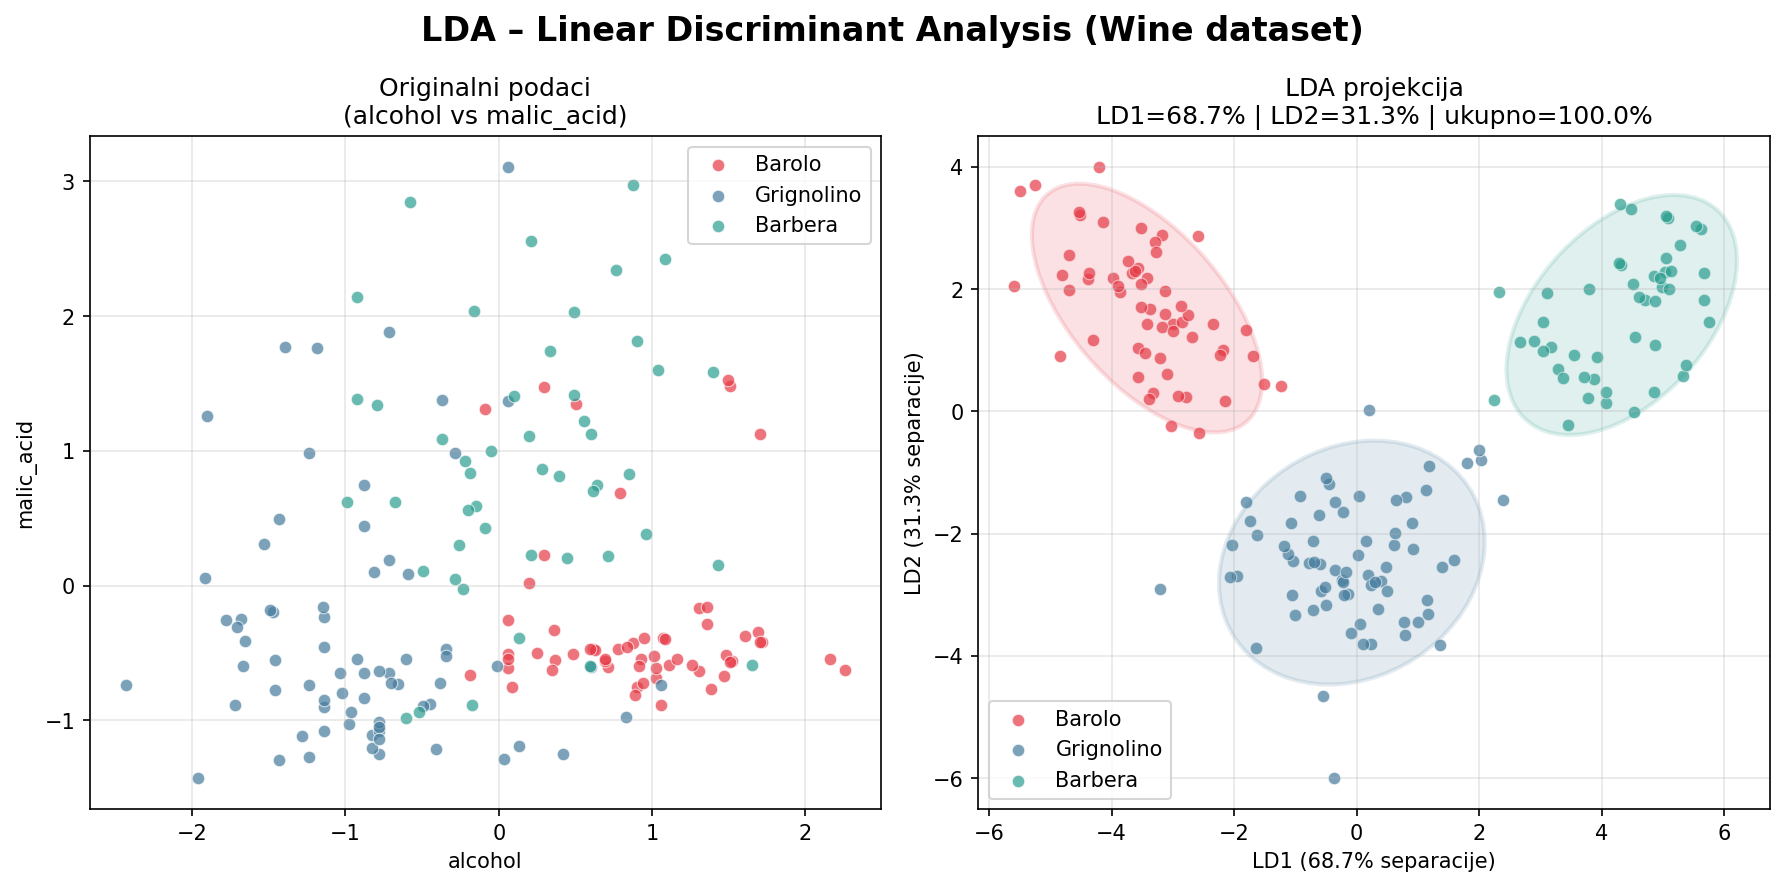
\includegraphics[width=\textwidth]{02_lda_wine.png}
		\caption{LDA на Wine скупу: оригинални подаци (лијево) и LDA пројекција (десно) са елипсама поузданости. Класе су знатно боље раздвојене него код PCA.}
		\label{fig:lda_wine}
	\end{figure}
	
	Слично као код PCA, и код LDA можемо погледати колико свака карактеристика доприноси појединој дискриминанти. На слици \ref{fig:lda_scalings} приказана је топлотна мапа тих вриједности за LD1 и LD2. Са мапе се види да прву дискриминанту (LD1) највише одређују флавоноиди ($-1{,}65$), пролин ($-0{,}85$) и OD280/OD315 ($-0{,}82$), док на другу дискриминанту (LD2) највише утичу пролин ($0{,}90$), алкохол ($0{,}71$) и пепео ($0{,}64$). То значи да LDA најјаче користи ове карактеристике како би раздвојио сорте вина.
	
	\begin{figure}[H]
		\centering
		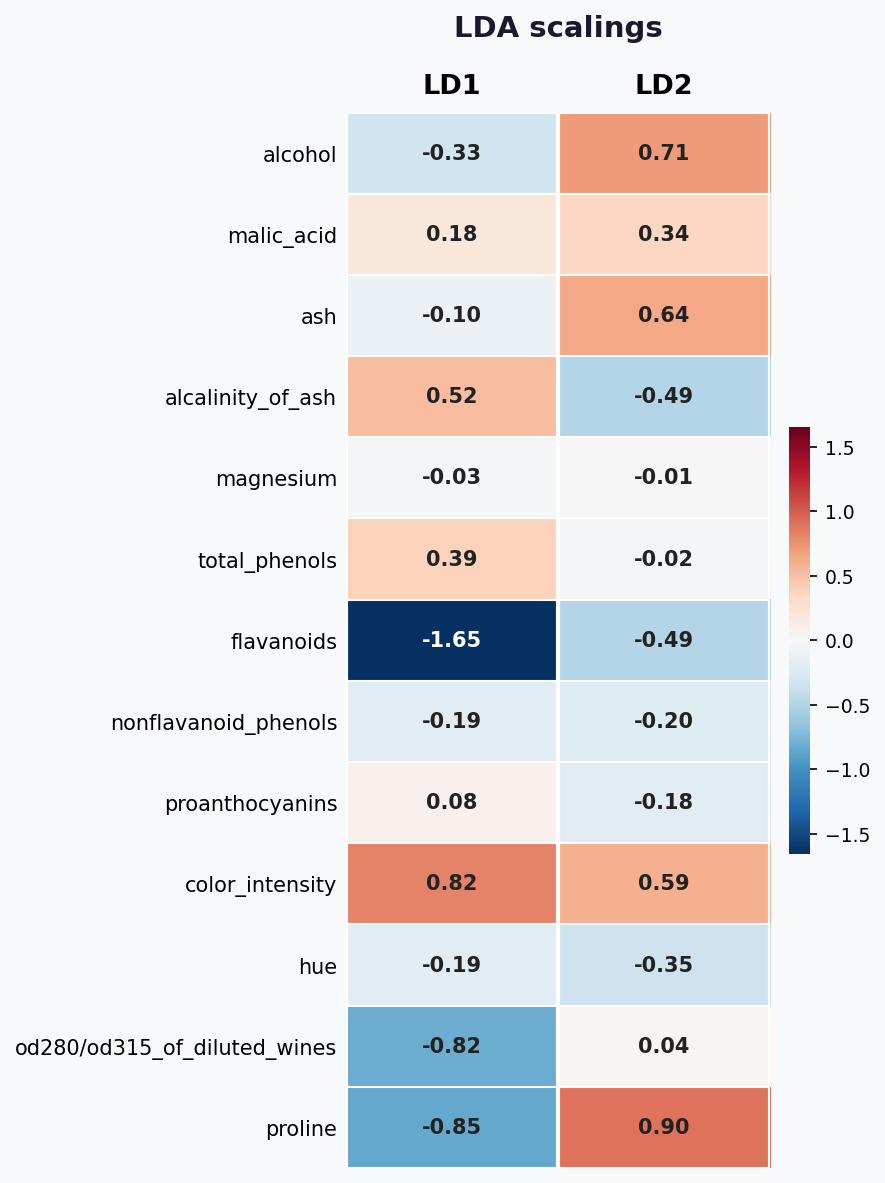
\includegraphics[width=7cm]{06b_lda_scalings.png}
		\caption{Топлотна мапа доприноса сваке карактеристике дискриминантама LD1 и LD2 код LDA.}
		\label{fig:lda_scalings}
	\end{figure}
	
	
	\subsubsection{Мјера сепарабилности: inter/intra однос}
	
	До сада смо о квалитету пројекција причали углавном на основу изгледа графика. Како бисмо то изразили и бројем, користимо однос расипања између класа и расипања унутар класа, познат као inter/intra однос:
	\begin{equation} \label{eq:fisher_score}
		J = \frac{S_B}{S_W} \quad.
	\end{equation}
	Идеја је иста као код Фишеровог критеријума: у бројиоцу је удаљеност између класа, а у имениоцу распршеност унутар класа. Зато већи однос $J$ значи да су класе истовремено боље раздвојене и компактније, односно да је пројекција квалитетнија.
	
	Овај однос смо израчунали за три случаја на Wine скупу:
	\begin{itemize}
		\item оригинални подаци (прве двије карактеристике): $J \approx 0{,}35$;
		\item PCA пројекција (двије компоненте): $J \approx 0{,}80$;
		\item LDA пројекција (двије компоненте): $J \approx 11{,}5$.
	\end{itemize}
	Резултати јасно показују колика је разлика. PCA донекле побољшава раздвојеност у односу на полазне податке, али LDA постиже готово 14 пута бољу сепарабилност од PCA. Овај резултат је и очекиван, јер LDA током рада користи информацију о класама, док PCA о њима не зна ништа.
	
	
	\subsubsection{Ограничења LDA}
	
	Иако LDA даје одличне резултате на Wine скупу, она има једно важно ограничење. LDA претпоставља да се класе могу раздвојити правом линијом, односно линеарном границом. Када је граница између класа нелинеарна, LDA заказује. Осим тога, LDA се ослања на центре класа - ако различите класе имају исти или веома близак центар, метода нема на основу чега да их раздвоји. На слици \ref{fig:lda_fail} су приказана два таква случаја.
	
	\textbf{Концентрични кругови.} У првом примјеру једна класа представља унутрашњи прстен, а друга спољашњи прстен. Обје класе имају исти центар, па је расипање између класа једнако нули ($\mathbf{S}_B = \mathbf{0}$). Пошто LDA раздваја класе управо на основу удаљености њихових центара, овдје нема никакву информацију те их не може раздвојити.
	
	\textbf{XOR проблем.} У другом примјеру класе су распоређене дијагонално, тако да се смјењују по угловима. И овдје све класе имају готово исти центар, па LDA поново не може да пронађе праву линију која би их раздвојила.
	
	У оба случаја видимо исту слабост: пошто LDA гледа само центре класа и тражи линеарну границу, не успијева да раздвоји класе чија је структура нелинеарна. За такве случајеве погодније су нелинеарне методе, о којима ће бити ријечи у наредном поглављу.
	
	\begin{figure}[H]
		\centering
		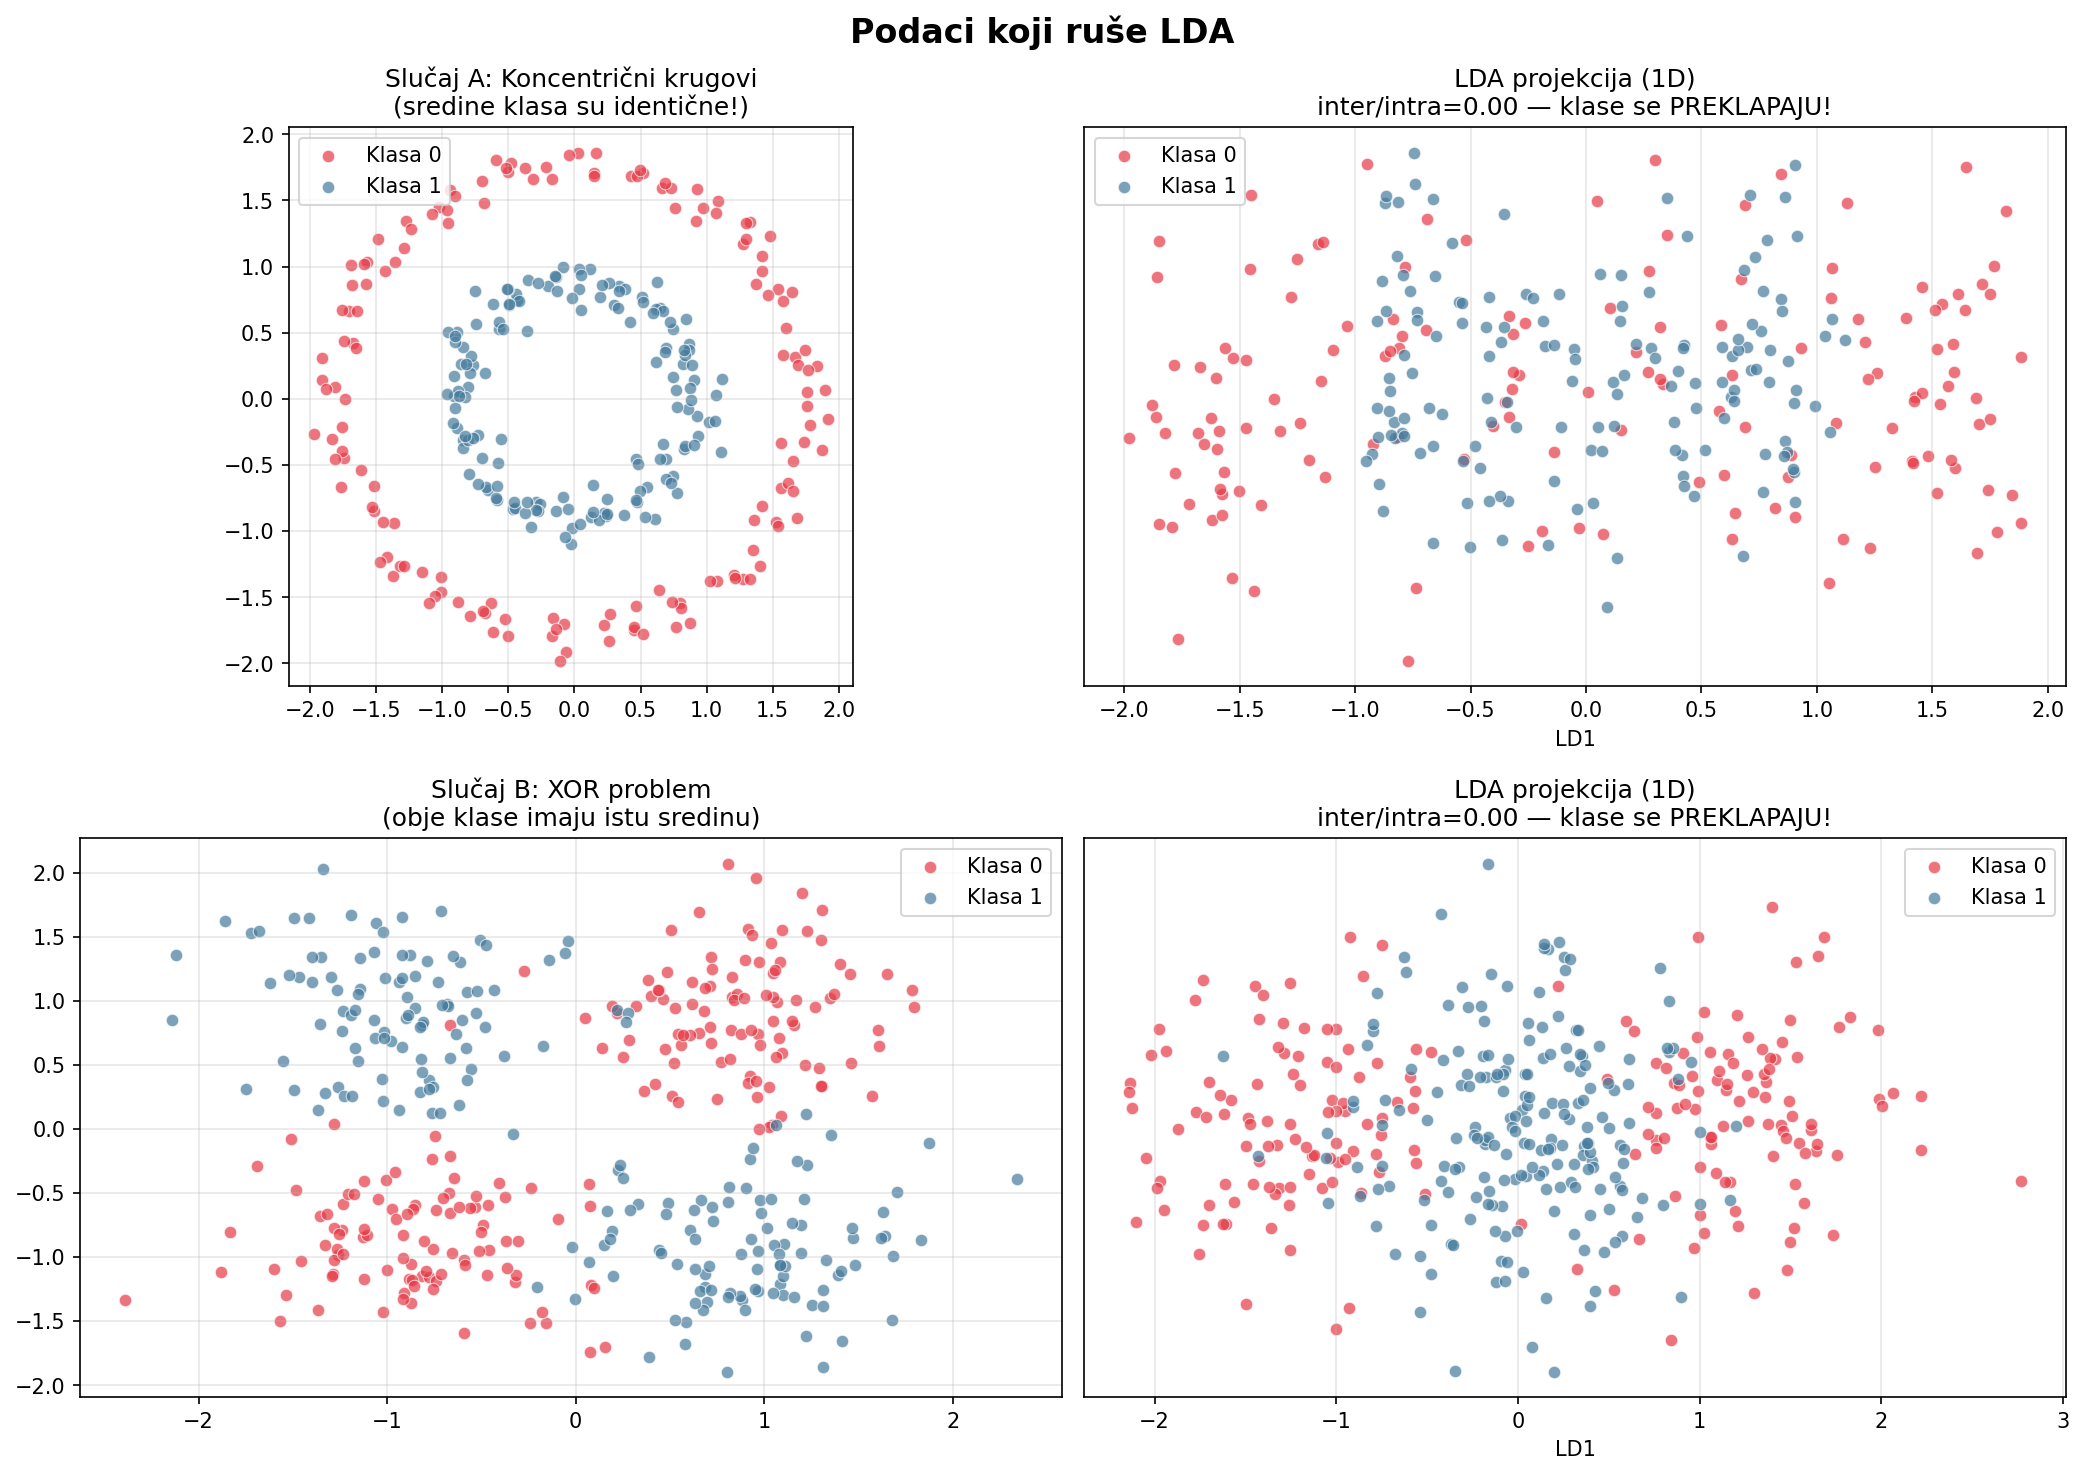
\includegraphics[width=\textwidth]{04_lda_failures.png}
		\caption{Случајеви гдје LDA заказује: концентрични кругови (А) и XOR проблем (Б). У оба случаја LDA пројицира класе у исту тачку јер су центроиди идентични.}
		\label{fig:lda_fail}
	\end{figure}
	
	
	\subsubsection{Када LDA надмашује PCA}
	
	Претходни примјери показали су случајеве у којима LDA заказује. Постоје, међутим, и ситуације у којима LDA даје знатно боље резултате од PCA. Такав примјер приказан је на слици \ref{fig:pca_fail_lda_win}. На лијевом панелу виде се полазни подаци: двије класе су јасно раздвојене по хоризонтали (дуж $x$ осе), али је варијанса у том правцу мања од варијансе дуж $y$ осе. По вертикали (дуж $y$ осе) подаци су веома распршени, али у том правцу нема никакве разлике међу класама - то је шум.
	
	Пошто PCA бира правац са највећом варијансом, она бира баш $y$ осу, односно правац шума. Када податке пројектује на тај правац, обје класе се потпуно измијешају и раздвојеност се губи (средњи панел на слици). LDA, с друге стране, не гледа варијансу већ раздвојеност класа. Она препознаје да корисна информација лежи дуж $x$ осе, иако је тамо варијанса мања, па податке пројектује баш на тај правац. Због тога класе остају јасно раздвојене (десни панел).
	
	Разлика је видљива и бројчано: inter/intra однос код PCA пројекције износи свега $0{,}002$, док код LDA износи чак $12{,}029$. Овај примјер показује суштинску разлику између двију метода - PCA бира правце по количини варијансе, док LDA бира правце по томе колико добро раздвајају класе. Управо зато, када је циљ раздвајање класа, LDA често даје боље резултате од PCA.
	
	\begin{figure}[H]
		\centering
		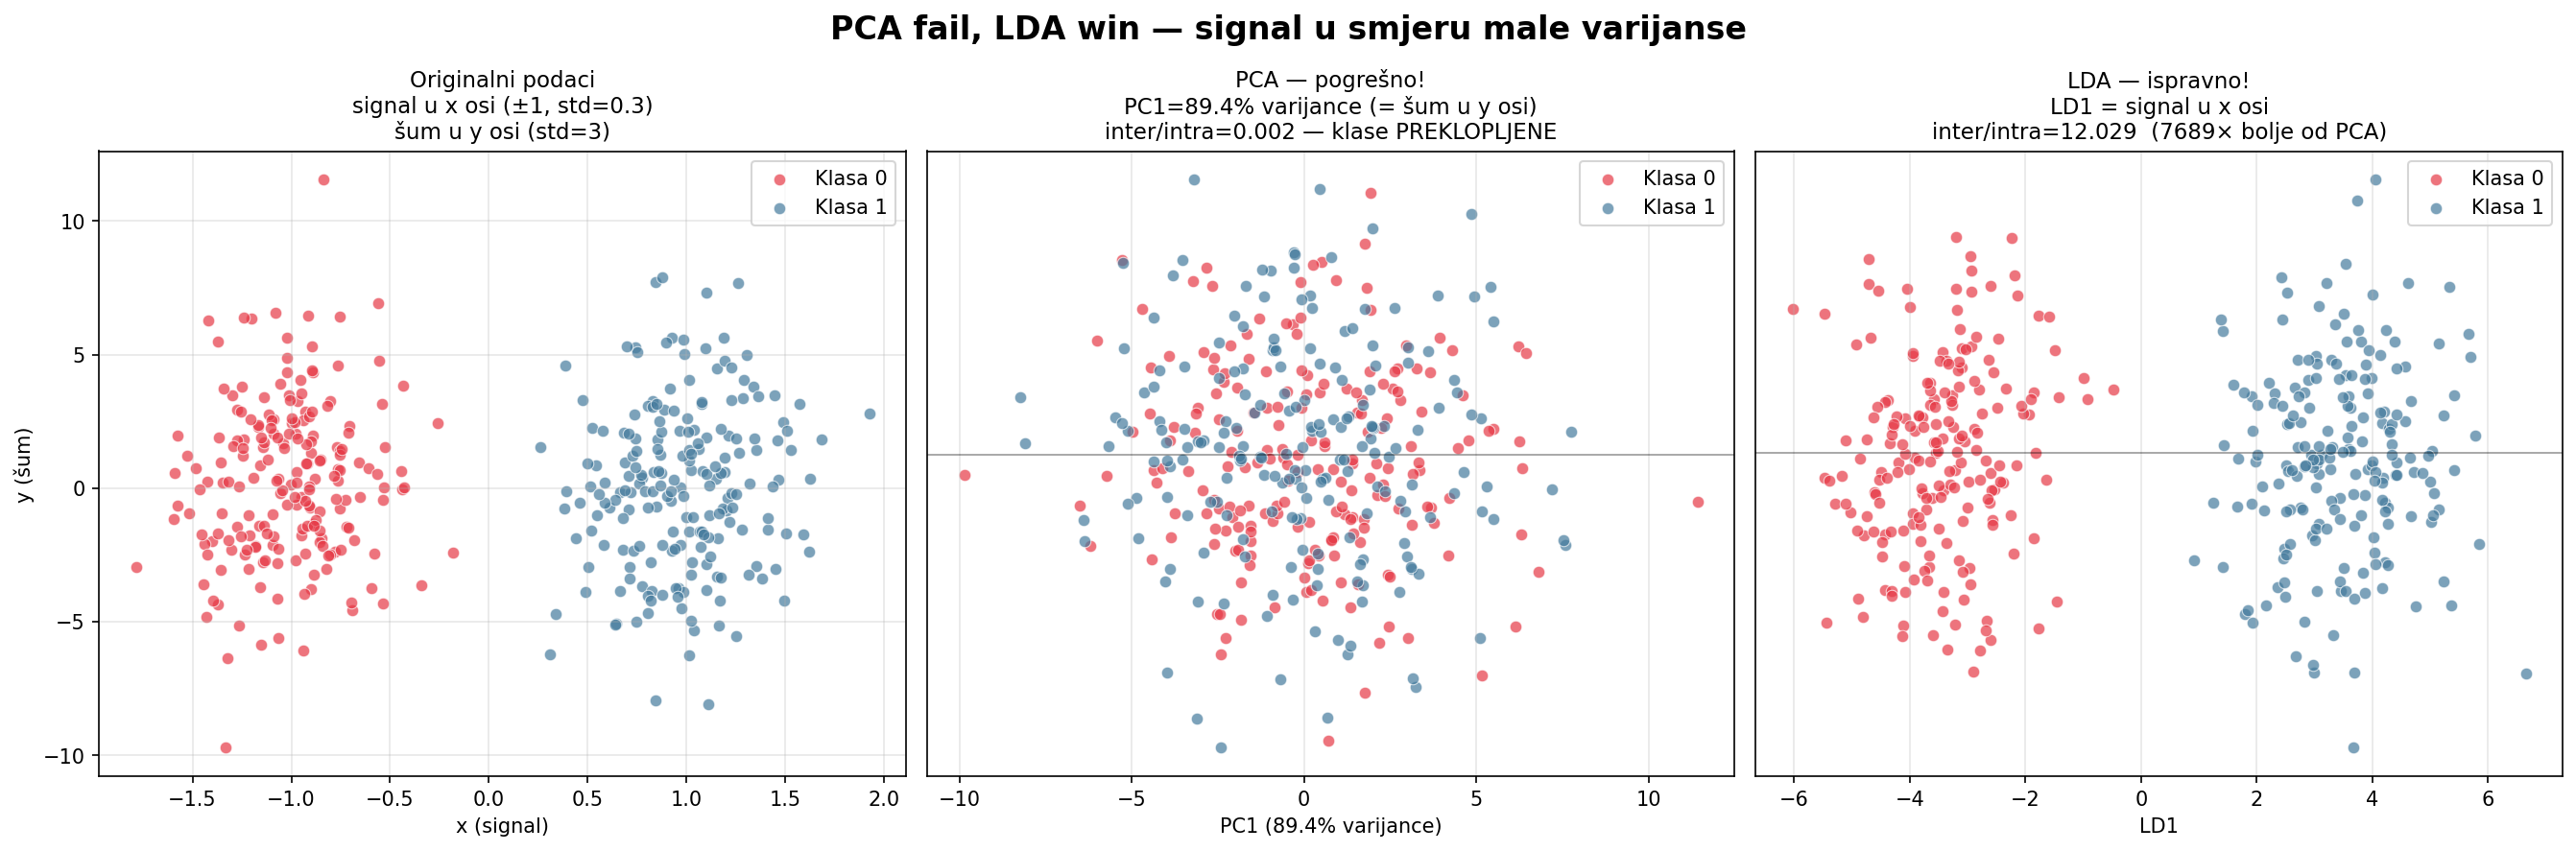
\includegraphics[width=\textwidth]{05_pca_fail_lda_win.png}
		\caption{PCA заказује - LDA успијева: класе су раздвојене у правцу мале варијансе ($y$ оса), а шум је у правцу велике варијансе ($x$ оса). PCA бира правац шума и мијеша класе, док LDA исправно бира правац који раздваја класе.}
		\label{fig:pca_fail_lda_win}
	\end{figure}
	
	\clearpage
	
	
	\section{Нелинеарне методе смањења димензионалности}
	
	\subsection{t-SNE - Стохастичко уметање сусједних тачака}
	
	t-SNE (енгл. \textit{$t$-distributed Stochastic Neighbor Embedding}) је нелинеарна метода смањења димензионалности која се првенствено користи за визуализацију података високе димензионалности \cite{maaten2008}. Ради се о \textbf{ненадгледаној} методи, што значи да не користи ознаке класа, већ гледа искључиво сличност међу самим тачкама. За разлику од PCA и LDA, t-SNE не покушава да сачува општу, глобалну слику података. Умјесто тога, њен главни циљ је да сачува распоред блиских тачака - тачке које су близу једна другој у оригиналном простору треба да остану близу и у нискодимензионалном приказу. Другим ријечима, t-SNE се труди да оно што је слично остане заједно, чак и када податке пребаци у простор ниже димензије (најчешће двије или три димензије, ради лакше визуелизације).
	
	\subsubsection{Поступак}
	
	\textbf{Корак 1 - Вјероватноће сусједстава у високим димензијама.} У првом кораку t-SNE за сваки пар тачака одређује колико су оне блиске у оригиналном простору. Уместо да гледа само удаљеност, t-SNE блискост изражава преко вјероватноће. За двије тачке $i$ и $j$ рачуна се вјероватноћа $p_{j|i}$, која говори колика је шанса да би тачка $i$ изабрала тачку $j$ за свог сусједа. Што су двије тачке ближе, та вјероватноћа је већа, а што су даље она је мања. Ова вјероватноћа се рачуна помоћу Гаусове расподјеле са варијансом $\sigma_i^2$:
	\begin{equation} \label{eq:tsne_p}
		p_{j|i} = \frac{\exp\!\left(-\|\mathbf{x}_i - \mathbf{x}_j\|^2 / 2\sigma_i^2\right)}{\displaystyle\sum_{k \neq i} \exp\!\left(-\|\mathbf{x}_i - \mathbf{x}_k\|^2 / 2\sigma_i^2\right)}.
	\end{equation}
	У бројиоцу се налази вриједност која је велика када су тачке $i$ и $j$ близу, а мала када су далеко. У имениоцу је збир истих таквих вриједности за све остале тачке, чиме се резултат своди на вриједност између 0 и 1.
	
	\textbf{Корак 2 - Симетризација.} Вјероватноћа из претходног корака није симетрична - вриједност $p_{j|i}$ не мора бити једнака $p_{i|j}$, јер зависи од тога коју тачку посматрамо као полазну. Да би алгоритам био стабилнији, ове двије вриједности се спајају у једну заједничку вјероватноћу $p_{ij}$, тако што се узме њихов просјек:
	\begin{equation} \label{eq:tsne_sym}
		p_{ij} = \frac{p_{j|i} + p_{i|j}}{2n}.
	\end{equation}
	На тај начин добијамо симетричну вриједност која подједнако важи за оба смјера, односно $p_{ij} = p_{ji}$.
	
	\textbf{Корак 3 - $t$-расподјела у нискодимензионалном простору.} До сада смо блискост тачака рачунали у оригиналном простору. Сада исто радимо и у новом, нискодимензионалном простору у који пребацујемо податке. За сваки пар тачака $i$ и $j$ рачуна се вјероватноћа $q_{ij}$, али се овдје умјесто Гаусове користи користи Студентова $t$-расподјела (енгл. \textit{Student's $t$-distribution}) са једним степеном слободе
	\begin{equation} \label{eq:tsne_q}
		q_{ij} = \frac{\left(1 + \|\mathbf{y}_i - \mathbf{y}_j\|^2\right)^{-1}}{\displaystyle\sum_{k \neq l} \left(1 + \|\mathbf{y}_k - \mathbf{y}_l\|^2\right)^{-1}}.
	\end{equation}
	Разлог за избор баш ове расподјеле лежи у њеном облику: она се према крајевима спушта спорије него Гаусова, па удаљеним тачкама додјељује веће вриједности. То удаљеним тачкама оставља више простора у приказу, чиме се спречава да се велики број тачака нагомила у средини - појава позната као ефекат ,,гужве у центру''.
	
	\textbf{Корак 4 - Минимизација KL дивергенције.} У претходним корацима добили смо двије расподјеле вјероватноће: расподјелу $P$, која описује блискост тачака у оригиналном простору, и расподјелу $Q$, која описује њихову блискост у новом, нискодимензионалном приказу. Циљ t-SNE је да ове двије расподјеле буду што сличније, односно да распоред тачака у приказу што вјеродостојнији оригиналу. Колико се оне разликују мјери се такозваном KL дивергенцијом:
	\begin{equation} \label{eq:tsne_kl}
		\text{KL}(P \| Q) = \sum_{i \neq j} p_{ij} \log\frac{p_{ij}}{q_{ij}}.
	\end{equation}
	Што је вриједност KL дивергенције мања, то су расподјеле $P$ и $Q$ сличније. Алгоритам зато постепено помјера тачке у приказу, користећи градијентни спуст, све док ова вриједност не постане што мања. Када се поступак заврши, блиске тачке из оригиналног простора остају блиске и у коначном приказу.
	
	
	\subsubsection{Матрице у t-SNE}
	
	За разлику од PCA и LDA, t-SNE не ради са матрицом коваријанси нити са матрицама расипања, већ са двије матрице вјероватноћа које описују блискост тачака. Овдје је укратко објашњено шта свака од њих представља.
	
	\textbf{$\mathbf{P}$ - Матрица вјероватноћа сусједстава у високим димензијама} (димензије $n \times n$, тј. $178 \times 178$). Ова матрица описује блискост тачака у оригиналном простору. Њен елемент $p_{ij}$ говори колика је вјероватноћа да би тачка $i$ изабрала тачку $j$ за свог сусједа. Блиске тачке имају високу вриједност $p_{ij}$, а удаљене тачке вриједност близу нуле. Пошто описује односе међу свих $n$ тачака, матрица има димензију $n \times n$, а на дијагонали су нуле (јер тачка није сама себи сусјед).
	
	\textbf{$\mathbf{Q}$ - Матрица вјероватноћа сусједстава у нискодимензионалном простору} (димензије $n \times n$). Ова матрица има исти облик и исто значење као $\mathbf{P}$, али се односи на нови, нискодимензионални приказ у који су тачке пребачене. Разлика је у томе што се овдје умјесто Гаусове користи Студентова $t$-расподјела. Управо се $\mathbf{P}$ и $\mathbf{Q}$ пореде током рада алгоритма, а циљ је да буду што сличније.
	
	\textbf{$\mathbf{Y}$ - Матрица нових координата} (димензије $n \times 2$, тј. $178 \times 2$ за приказ у двије димензије). Ово је крајњи резултат t-SNE, у коме сваки ред садржи нове координате једне тачке. Важно је напоменути да саме вриједности координата немају физичко значење - битан је само међусобни распоред тачака, односно које су близу, а које далеко.
	
	
	\subsubsection{Хиперпараметар: Perplexity}
	
	Прије него што покренемо t-SNE, потребно је да сами задамо неке вриједности које управљају његовим радом - такве вриједности називамо хиперпараметрима. Код t-SNE најважнији хиперпараметар је \textit{perplexity}. Он одређује колико сусједних тачака свака тачка ,,узима у обзир'' када се рачуна блискост, односно колико широко t-SNE гледа око сваке тачке. Његове вриједности се обично крећу између 5 и 50, горњи ред).
	
	Избор ове вриједности значајно утиче на изглед коначног приказа:
	\begin{itemize}
		\item \textbf{мала вриједност (нпр. 5):} тачка гледа само своје најближе сусједе, па се појављују ситне и расцијепкане групе;
		\item \textbf{средња вриједност (нпр. 30):} постиже се равнотежа између локалне и опште структуре, па се ова вриједност најчешће користи у пракси;
		\item \textbf{велика вриједност (нпр. 50 и више):} тачка гледа много сусједа, па групе постају шире и мање јасно раздвојене.
	\end{itemize}
	
	Са слике \ref{fig:hyperparams} се види управо то - иста група података изгледа потпуно другачије када се користе различите вриједности \textit{perplexity}, из овога видимо да овај хиперпараметар треба пажљиво изабрати.
	
	\begin{figure}[H]
		\centering
		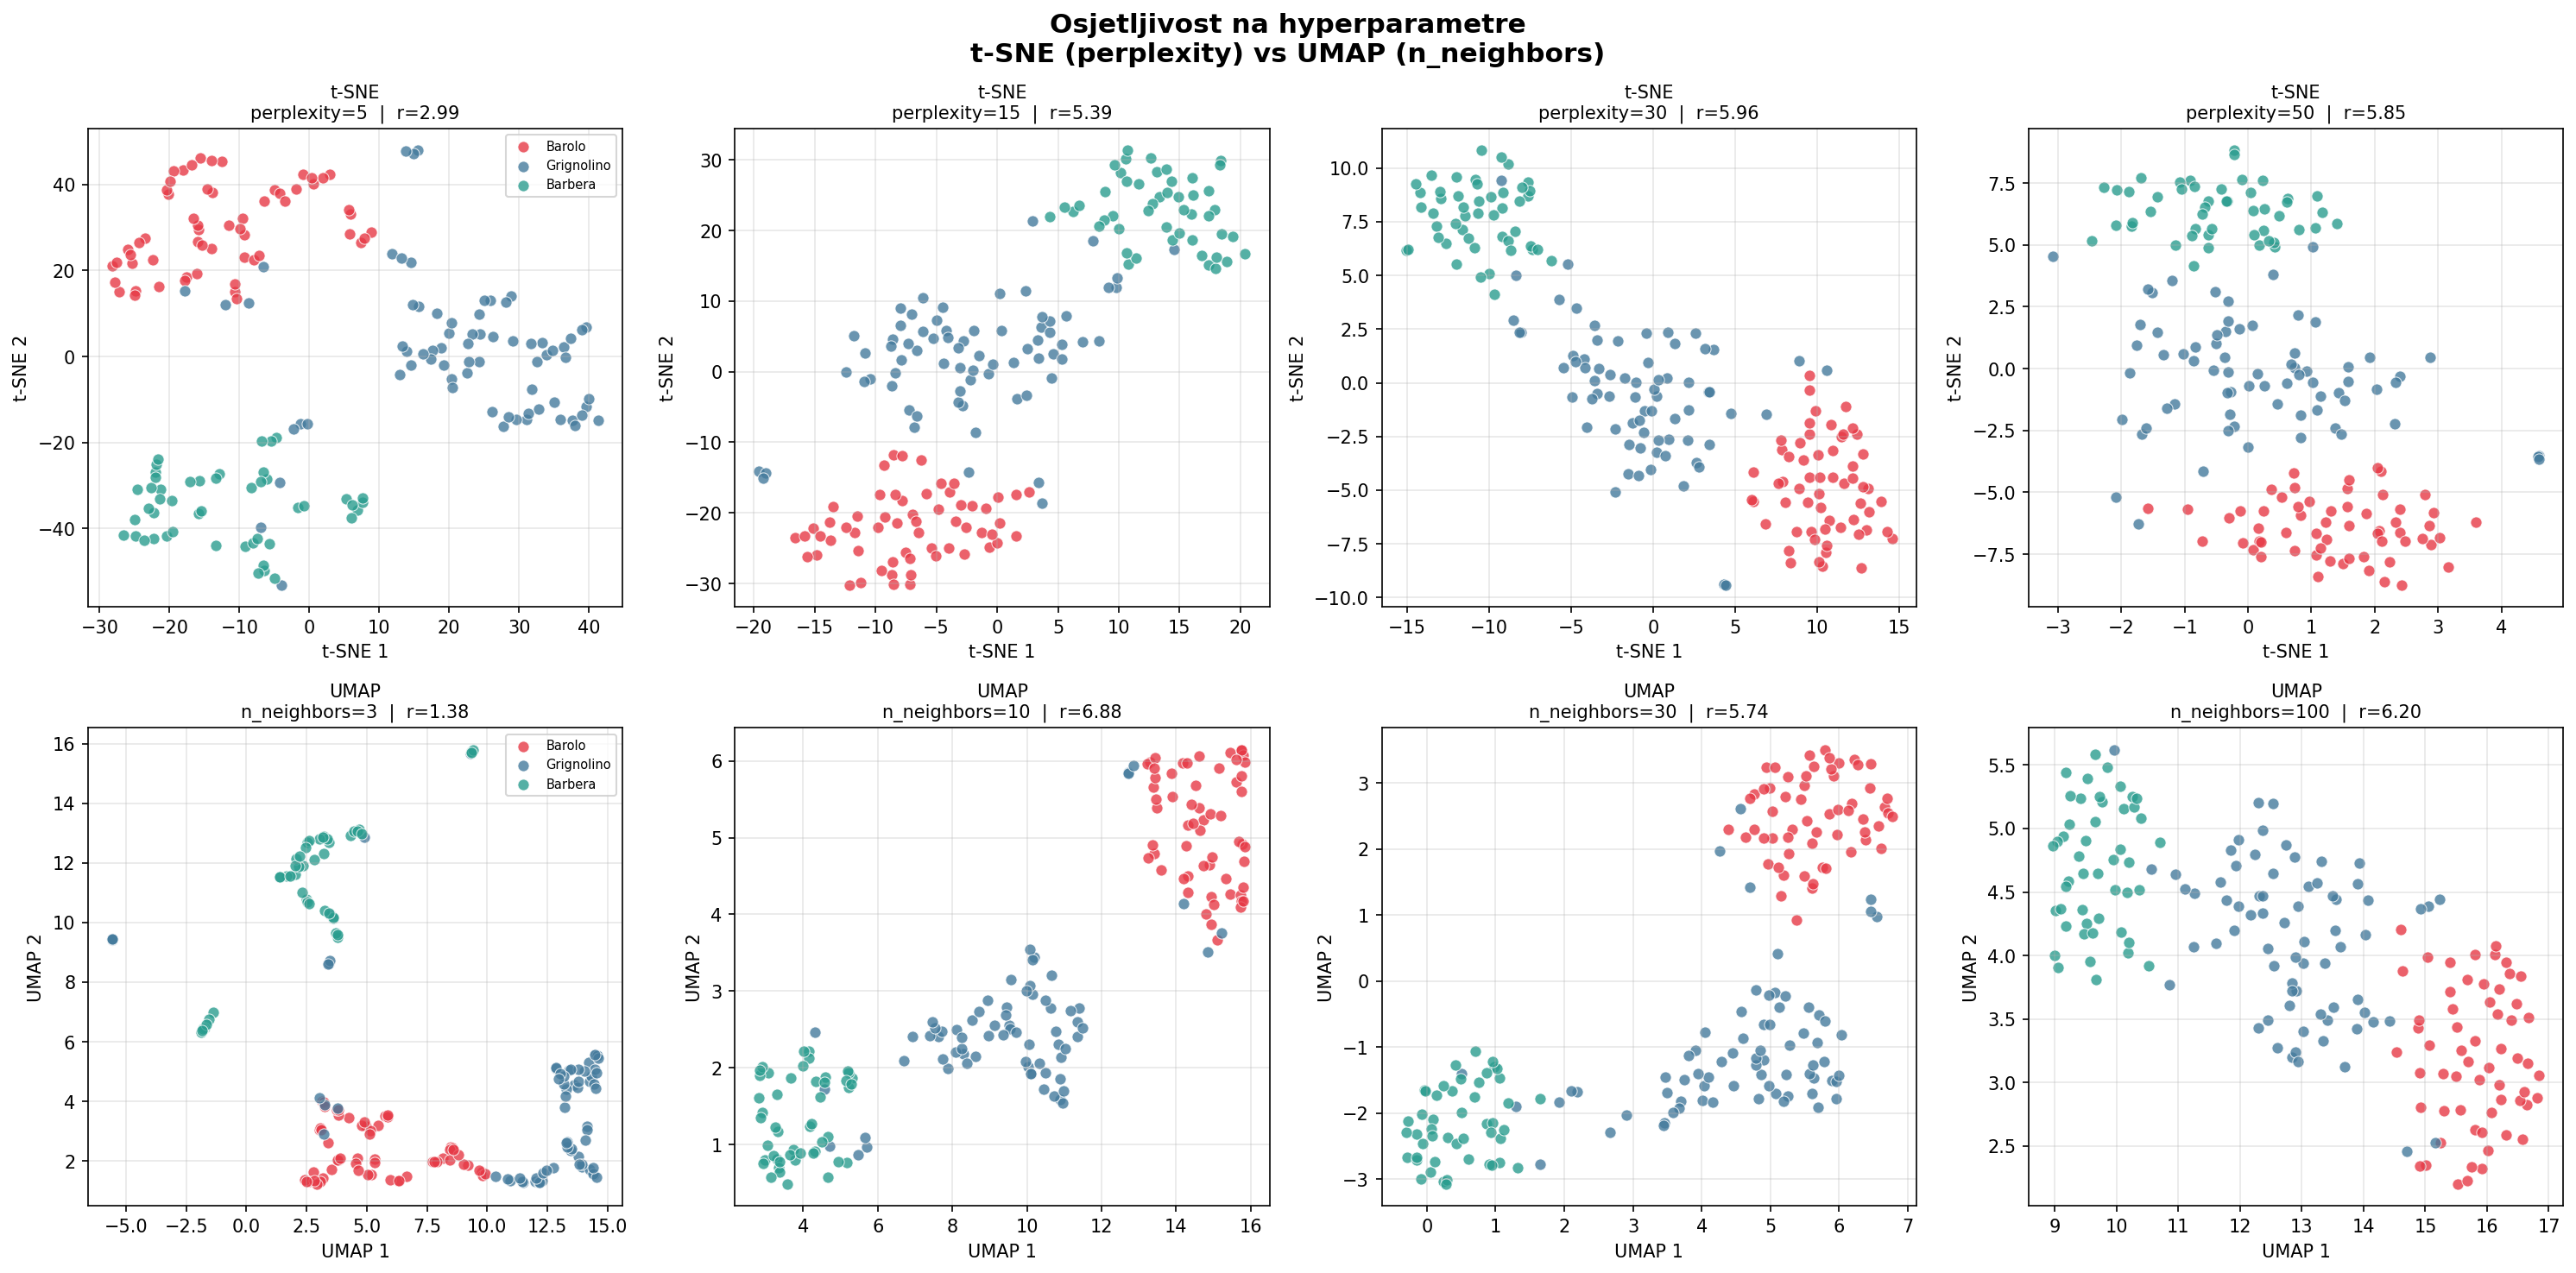
\includegraphics[width=\textwidth]{t03_hyperparametri.png}
		\caption{Осјетљивост на хиперпараметре: t-SNE (горњи ред) са \textit{perplexity} = 5, 15, 30, 50 и UMAP (доњи ред) са $n\_neighbors$ = 3, 10, 30, 100. Уочљиво је да различите вриједности хиперпараметра значајно мијењају изглед пројекције.}
		\label{fig:hyperparams}
	\end{figure}
	
	
	\subsubsection{t-SNE пројекција Wine скупа}
	
	Када t-SNE примијенимо на Wine скуп, добијамо приказ у коме су три сорте вина врло јасно раздвојене (слика \ref{fig:tsne_wine}). Лијеви панел приказује саму пројекцију, на којој се јасно виде три групе (Barolo, Grignolino и Barbera), свака обухваћена својом елипсом поузданости. Десни панел приказује \textit{inter/intra} однос, којим се бројчано мјери квалитет раздвајања класа: код t-SNE он износи $5{,}96$, што је знатно више него код PCA ($3{,}41$), а близу вриједности коју постиже надгледана LDA ($6{,}61$). То значи да t-SNE, иако не користи податке о класама, успијева да сорте раздвоји готово једнако добро као LDA.
	
	Осе на t-SNE графику немају физичко значење - за разлику од PCA, гдје осе одговарају главним компонентама, овдје бројеви на осама сами по себи ништа не значе. Битан је једино међусобни распоред тачака, односно које су групе близу, а које далеко. Због тога t-SNE користимо за визуелно откривање структуре у подацима, али не и за прецизно мјерење удаљености међу тачкама.
	
	\begin{figure}[H]
		\centering
		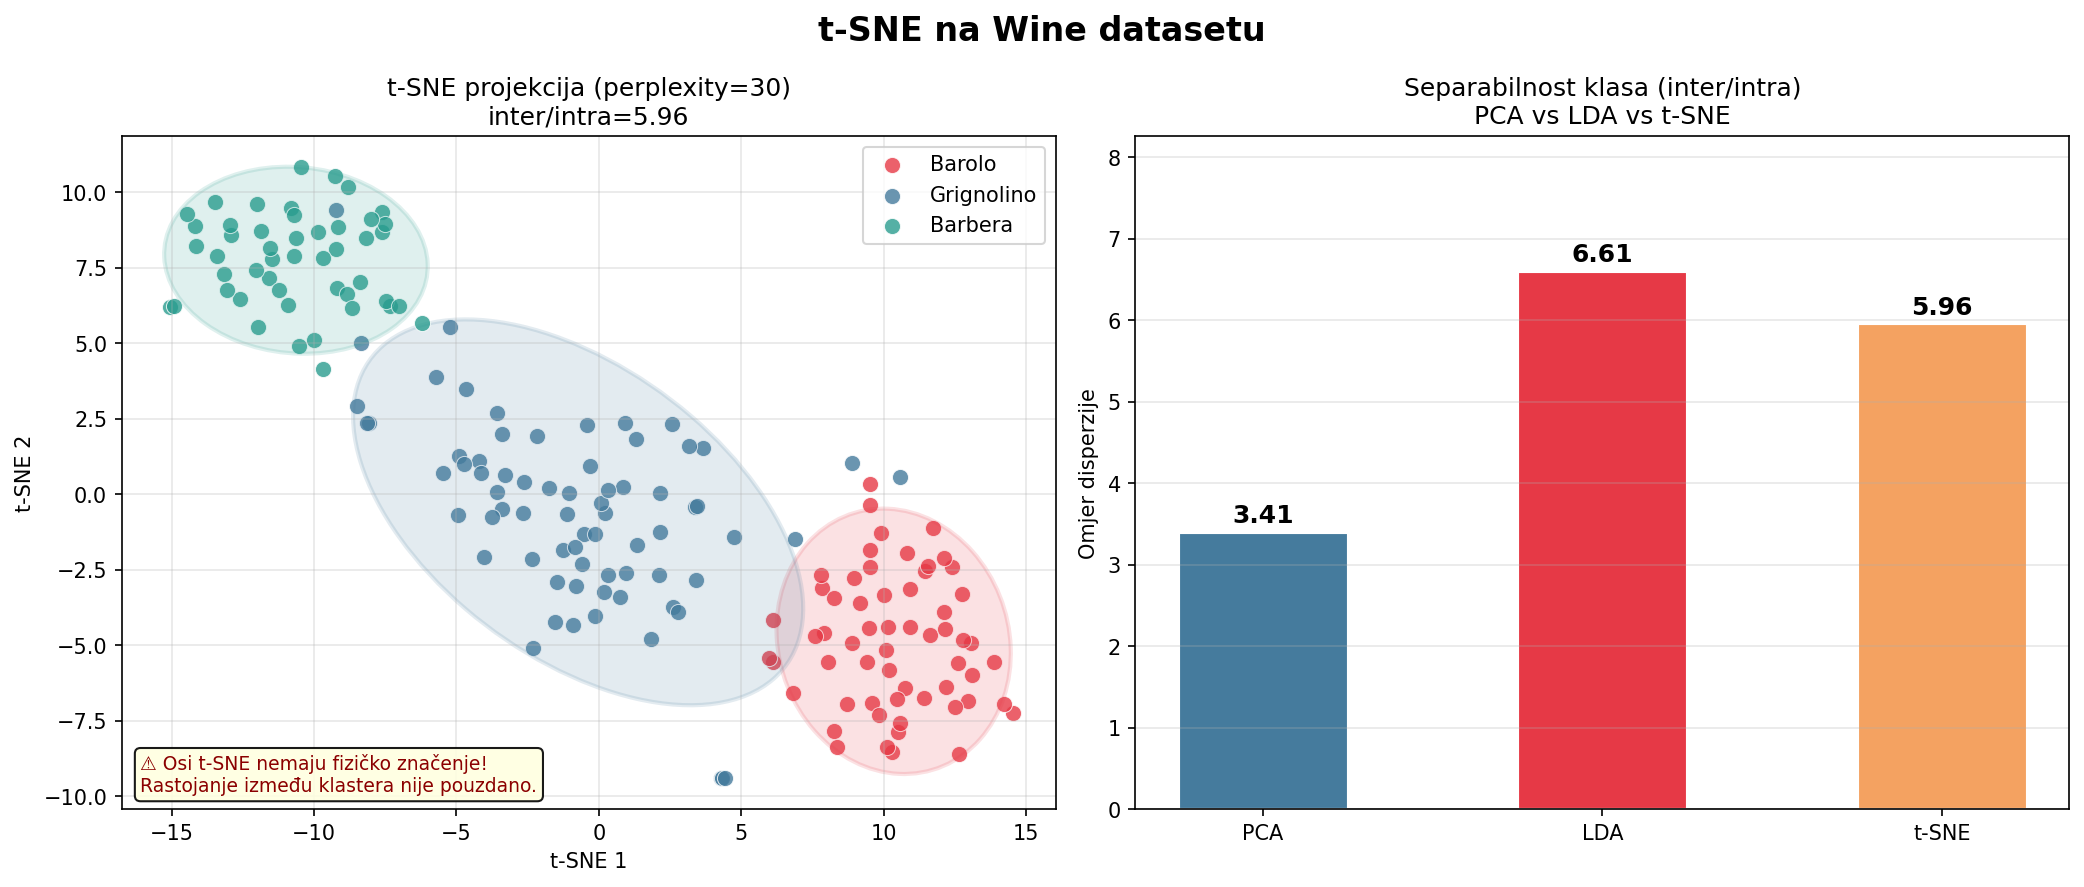
\includegraphics[width=\textwidth]{t01_tsne_wine.png}
		\caption{t-SNE на Wine скупу: пројекција са елипсама поузданости (лијево) и поређење \textit{inter/intra} односа за PCA, LDA и t-SNE (десно).}
		\label{fig:tsne_wine}
	\end{figure}
	
	
	\subsubsection{Ограничења t-SNE}
		
	Т-SNE је веома користан за визуализацију, али има и неколико важних ограничења:
	\begin{itemize}
		\item \textbf{Осе немају физичко значење.} Бројеви на осама t-SNE графика ништа не значе сами по себи - већ је битан само међусобни распоред тачака, а не њихове конкретне координате.
		\item \textbf{Удаљеност међу групама није поуздана.} Двије групе које на t-SNE приказу изгледају веома удаљено не морају заиста бити далеко и у оригиналном простору. Осим тога, t-SNE изобличи и релативне величине група, па оне на приказу не одговарају стварном броју тачака (слика \ref{fig:tsne_izuzeci}). Зато се из t-SNE графика не смије закључивати колико су групе међусобно удаљене нити колике су заправо.
		\item \textbf{Може приказати лажну структуру.} t-SNE понекад ,,пронађе'' групе чак и тамо гдје их заправо нема, односно у потпуно насумичним подацима без икакве стварне структуре. Зато распоред тачака на t-SNE приказу треба узети са опрезом и не тумачити свако згуснуће као стварну групу.
		\item \textbf{Не подржава пројекцију нових тачака.} Једном истрениран модел не може директно да пресликава нове тачке - за сваку нову тачку алгоритам се мора поново покренути над свим подацима.
		\item \textbf{Спор је.} Због сложености $O(n^2)$ t-SNE постаје непрактичан за велике скупове података (преко $10\,000$ узорака).
		\item \textbf{Није детерминистичан.} Свако покретање може дати помало другачији резултат, јер алгоритам почиње од насумичног распореда тачака.
	\end{itemize}
	
	\begin{figure}[H]
		\centering
		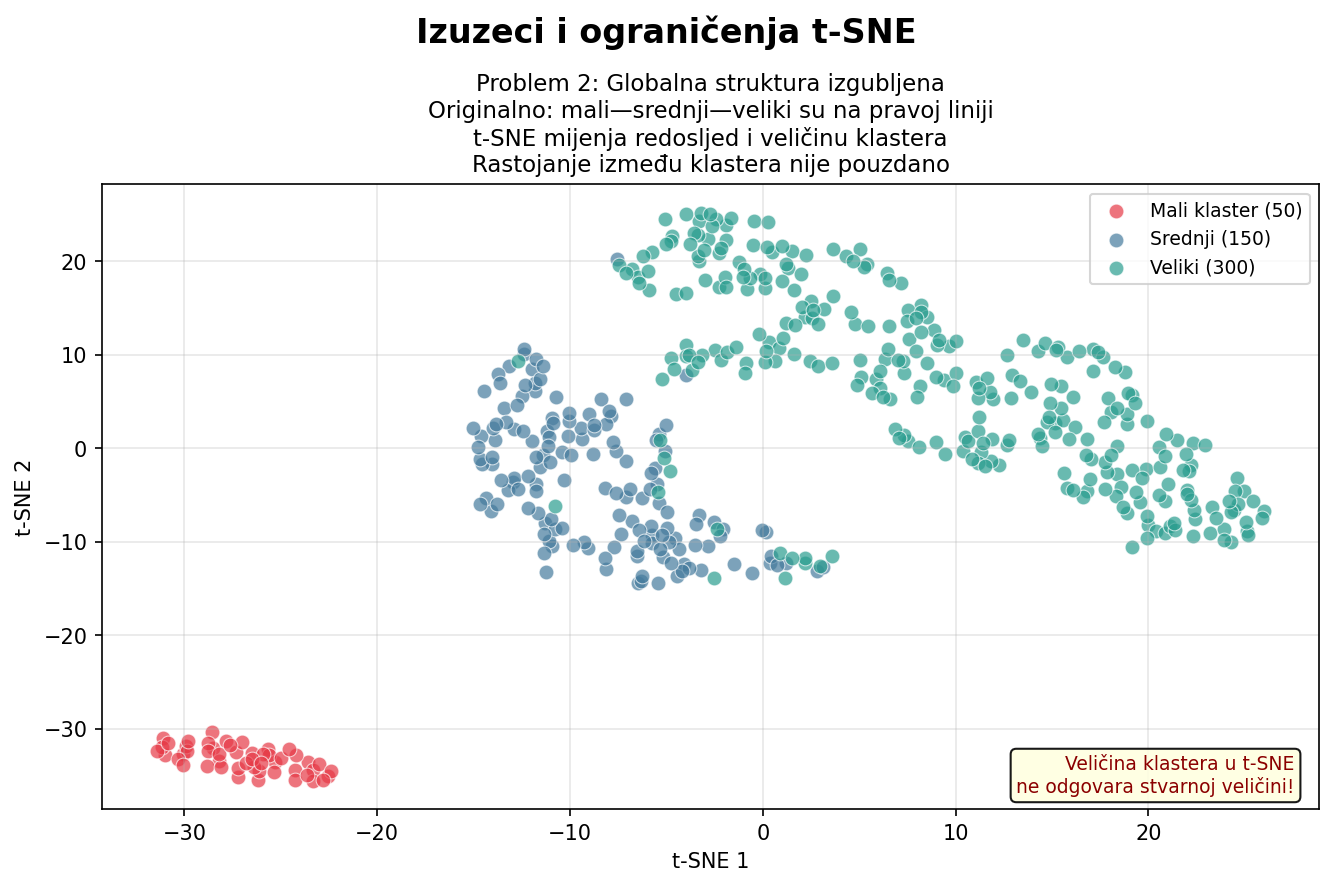
\includegraphics[width=10cm]{t06_izuzeci_tsne.png}
		\caption{Ограничења t-SNE: три групе које су у оригиналу биле поређане на правој линији t-SNE приказује измијењеног распореда и величине, па ни удаљеност ни величина група на приказу нису поуздане.}
		\label{fig:tsne_izuzeci}
	\end{figure}
	
	\clearpage
	
	
	\subsection{UMAP - Уједначена апроксимација многострукости}
	
	UMAP, Уједначена апроксимација многострукости (енгл. \textit{Uniform Manifold Approximation and Projection}) је новија нелинеарна метода смањења димензионалности \cite{mcinnes2018}. Као и t-SNE, ради се о \textbf{ненадгледаној} методи која не користи ознаке класа, већ гледа сличност међу самим тачкама и труди се да оно што је блиско у оригиналном простору остане блиско и у нискодимензионалном приказу.
	
	UMAP се заснива на сложеној математичкој теорији (Ријемановој геометрији и топологији), али за разумијевање његове примјене није неопходно улазити у ту теорију \cite{coenen2019}. Довољно је знати да UMAP, слично t-SNE, чува локалну структуру података, односно распоред блиских тачака. У пракси UMAP даје резултате сличне t-SNE, али уз неколико предности: знатно је бржи, боље чува општу (глобалну) слику података, и може да пресликава нове тачке без поновног покретања над цијелим скупом. Управо због овога се UMAP често користи као бржа и практичнија алтернатива t-SNE методи.
	
	
	\subsubsection{Поступак}
	
	UMAP полази од претпоставке да подаци, иако описани великим бројем карактеристика, заправо леже на некој глаткој, закривљеној површини унутар тог простора. Таква површина се назива многострукост (енгл. \textit{manifold}). Циљ UMAP-а је да пронађе приказ у мање димензија који што вјерније чува облик и структуру те површине, односно распоред тачака на њој.
	
	\textbf{Корак 1 - Изградња графа susjedstva.} UMAP најприје за сваку тачку пронађе њених $n\_neighbors$ најближих сусједа и повеже их линијама у мрежу (граф). Свака веза добија тежину која говори колико су двије тачке блиске - што су ближе, тежина је већа. На тај начин настаје мрежа која описује локалну структуру података, то јест које су тачке једна другој близу.
	Тежина везе између тачака $i$ и $j$ рачуна се као:
	\begin{equation} \label{eq:umap_weight}
		w_{ij} = \exp\!\left(\frac{-(d(x_i, x_j) - \rho_i)}{\sigma_i}\right),
	\end{equation}
	гдје је $d(x_i, x_j)$ удаљеност између тачака, $\rho_i$ удаљеност до најближег сусједа, а $\sigma_i$ параметар који се бира тако да свака тачка има уравнотежен број веза.
	
	\textbf{Корак 2 - Распоређивање тачака у мањем простору.} Затим UMAP покушава да исту ту мрежу нацрта у новом простору мање димензије. Тачке се распоређују тако да мрежа веза у новом приказу што вјерније одговара мрежи из оригиналног простора. Другим ријечима, тачке које су биле повезане и блиске остају блиске и у новом приказу.
	
	\textbf{Корак 3 - Дотјеривање распореда.} На крају UMAP постепено помјера тачке како би се два графа што боље поклопили. Ово дотјеривање се ради помоћу градијентног спуста, исте технике коју користи и t-SNE, све док распоред тачака не постане што вјернији оригиналу.UMAP минимизује бинарну крос-ентропију између тежина веза у оригиналном и новом простору:
	\begin{equation} \label{eq:umap_loss}
		C = \sum_{i \neq j} \left[ w_{ij} \log\frac{w_{ij}}{v_{ij}} + (1 - w_{ij}) \log\frac{1 - w_{ij}}{1 - v_{ij}} \right],
	\end{equation}
	гдје су $w_{ij}$ тежине у оригиналном, а $v_{ij}$ тежине у новом простору.
	
	
	\subsubsection{Матрице у UMAP}
	
	Слично t-SNE, и UMAP не ради са матрицом коваријанси, већ са графовима који описују блискост тачака, а који се могу представити као матрице. Овдје је укратко објашњено шта свака од њих представља.
	
	\textbf{$\mathbf{A}_{high}$ - Матрица тежина сусједског графа у високим димензијама} (димензије $n \times n$). Ова матрица описује блискост тачака у оригиналном простору. Њен елемент говори колико је јака веза између двије тачке - што су ближе, вриједност је већа. За разлику од t-SNE матрице $\mathbf{P}$, која је густа (свака тачка је повезана са свим осталим), код UMAP-а је свака тачка повезана само са својих $n\_neighbors$ најближих сусједа. Зато је ова матрица \textit{ретка}, односно највећи број њених елемената једнак је нули. Тежина везе се рачуна као:
	\begin{equation} \label{eq:umap_ahigh}
		A_{high,ij} = \exp\!\left(-\frac{d_{ij} - \rho_i}{\sigma_i}\right),
	\end{equation}
	гдје је $d_{ij}$ удаљеност између тачака $i$ и $j$, $\rho_i$ удаљеност до најближег сусједа, а $\sigma_i$ параметар који се бира тако да сваки чвор има уравнотежен број веза, у складу са задатим $n\_neighbors$.
	
	\textbf{$\mathbf{A}_{low}$ - Матрица тежина графа у нискодимензионалном простору} (димензије $n \times n$, такође ретка). Ова матрица има исто значење као претходна, али се односи на нови приказ у мање димензија. UMAP распоређује тачке тако да ова матрица што вјерније одговара матрици $\mathbf{A}_{high}$ из оригиналног простора. Њене тежине се рачунају као:
	\begin{equation} \label{eq:umap_alow}
		A_{low,ij} = \left(1 + a\,\|\mathbf{y}_i - \mathbf{y}_j\|^{2b}\right)^{-1},
	\end{equation}
	гдје су $a$ и $b$ параметри чије вриједности зависе од хиперпараметра $min\_dist$, који одређује колико ће тачке у приказу бити збијене или разбацане.
	
	\textbf{$\mathbf{Y}$ - Матрица нових координата} (димензије $n \times 2$, тј. $178 \times 2$ за приказ у двије димензије). Ово је крајњи резултат UMAP-а, у коме сваки ред садржи нове координате једне тачке. За разлику од t-SNE, UMAP памти научени модел, па може да пресликава и нове тачке које нису биле коришћене приликом учења, без поновног покретања над цијелим скупом.
	
	
	\subsubsection{Хиперпараметри UMAP-а}

	UMAP има два главна хиперпараметра којима се управља његовим радом: $n\_neighbors$ и $min\_dist$.
	
	\textbf{$n\_neighbors$ (типично 15).} Овај хиперпараметар одређује колико сусједа UMAP узима у обзир око сваке тачке, односно колико широко гледа при изградњи мреже. Мале вриједности значе да свака тачка гледа само своје најближе сусједе, па UMAP хвата ситну, локалну структуру. Веће вриједности значе да тачка гледа шире, па UMAP боље хвата општу, глобалну слику података (слика \ref{fig:hyperparams}, доњи ред). Утицај ове вриједности је сљедећи:
	\begin{itemize}
		\item $n\_neighbors = 2$--$5$: тачка гледа премало сусједа, па се групе распадају на ситне фрагменте и доминира локални шум;
		\item $n\_neighbors = 15$: постиже се равнотежа између локалне и глобалне структуре, па се ова вриједност најчешће користи;
		\item $n\_neighbors = 50$--$100$: тачка гледа много сусједа, па се добија глатка, општа слика, али се губи фина локална структура.
	\end{itemize}
	
	\textbf{$min\_dist$ (типично 0,1).} Овај хиперпараметар одређује колико близу тачке смију бити једна другој у коначном приказу. Мања вриједност значи да се тачке могу збити веома близу, па су групе компактније и гушће. Већа вриједност тачке држи размакнутима, па је пројекција разуђенија, а групе шире. Због тога $min\_dist$ не утиче на то које су тачке заједно, већ само на то колико ће бити збијене (слика \ref{fig:umap_izuzeci}).
	
	\begin{figure}[h]
		\centering
		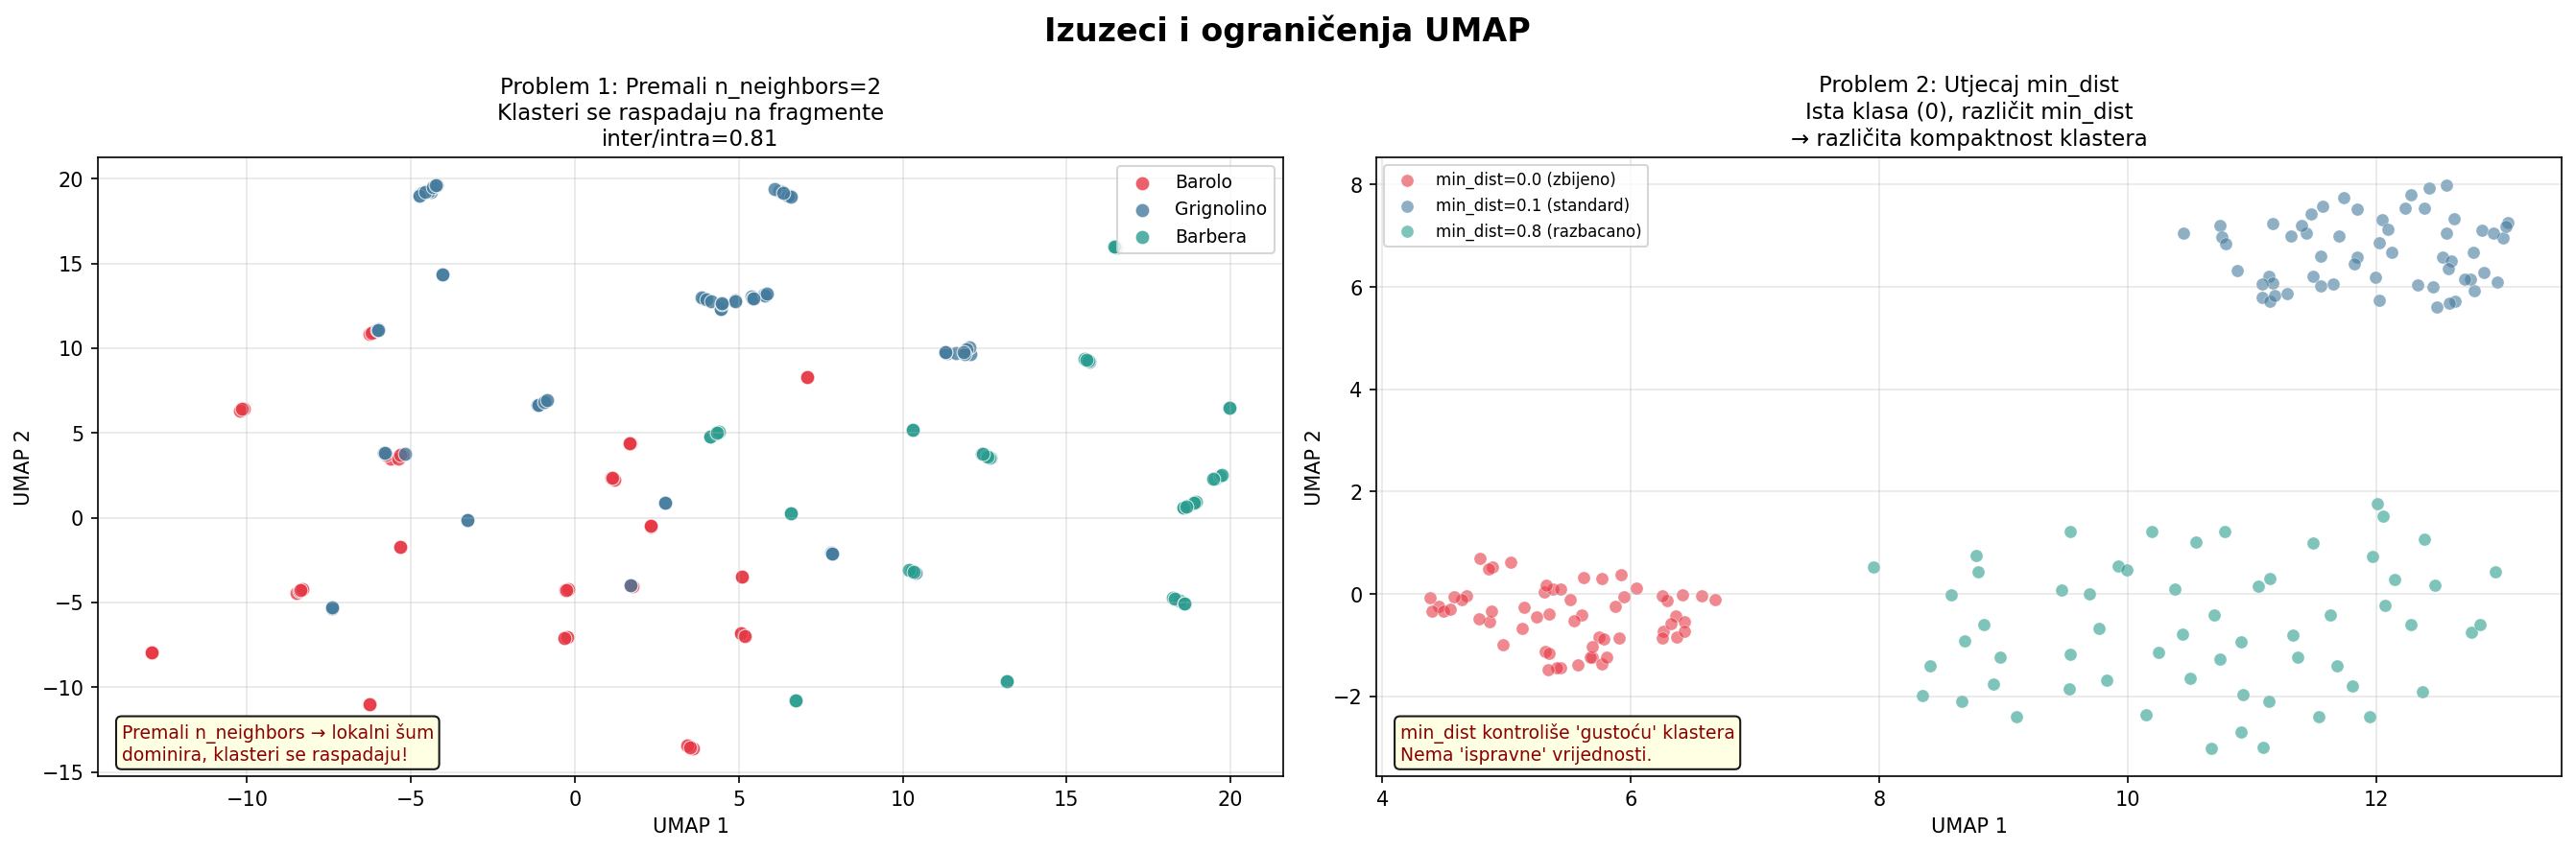
\includegraphics[width=\textwidth]{t07_izuzeci_umap.png}
		\caption{Ограничења UMAP-а: ефекат премалог $n\_neighbors = 2$ - групе се распадају на фрагменте (лијево); ефекат различитих вриједности $min\_dist$ на исту класу (десно).}
		\label{fig:umap_izuzeci}
	\end{figure}
	
	
	\subsubsection{UMAP пројекција Wine скупа}
	
	Када UMAP примијенимо на Wine скуп, добијамо приказ у коме су три сорте вина јасно раздвојене (слика \ref{fig:umap_wine}). Лијеви панел приказује саму пројекцију, на којој се виде три компактне и добро одвојене групе (Barolo, Grignolino и Barbera), свака обухваћена својом елипсом поузданости. Десни панел приказује \textit{inter/intra} однос за све четири методе. Код UMAP-а он износи $6{,}85$, што је највећа вриједност међу свим методама - већа чак и од надгледане LDA ($6{,}61$), а знатно већа од t-SNE ($5{,}96$) и PCA ($3{,}41$).
	
	Овај резултат показује да UMAP на Wine скупу постиже одличну визуелну раздвојеност класа, и то иако, као и t-SNE, не користи податке о класама. Уз то, UMAP ову раздвојеност постиже брже од t-SNE и уз могућност пресликавања нових тачака, што га чини погодним и за практичну примјену. Као и код t-SNE, треба имати на уму да осе на UMAP графику немају физичко значење - битан је само међусобни распоред тачака, а не саме вриједности координата.
	
	\begin{figure}[h]
		\centering
		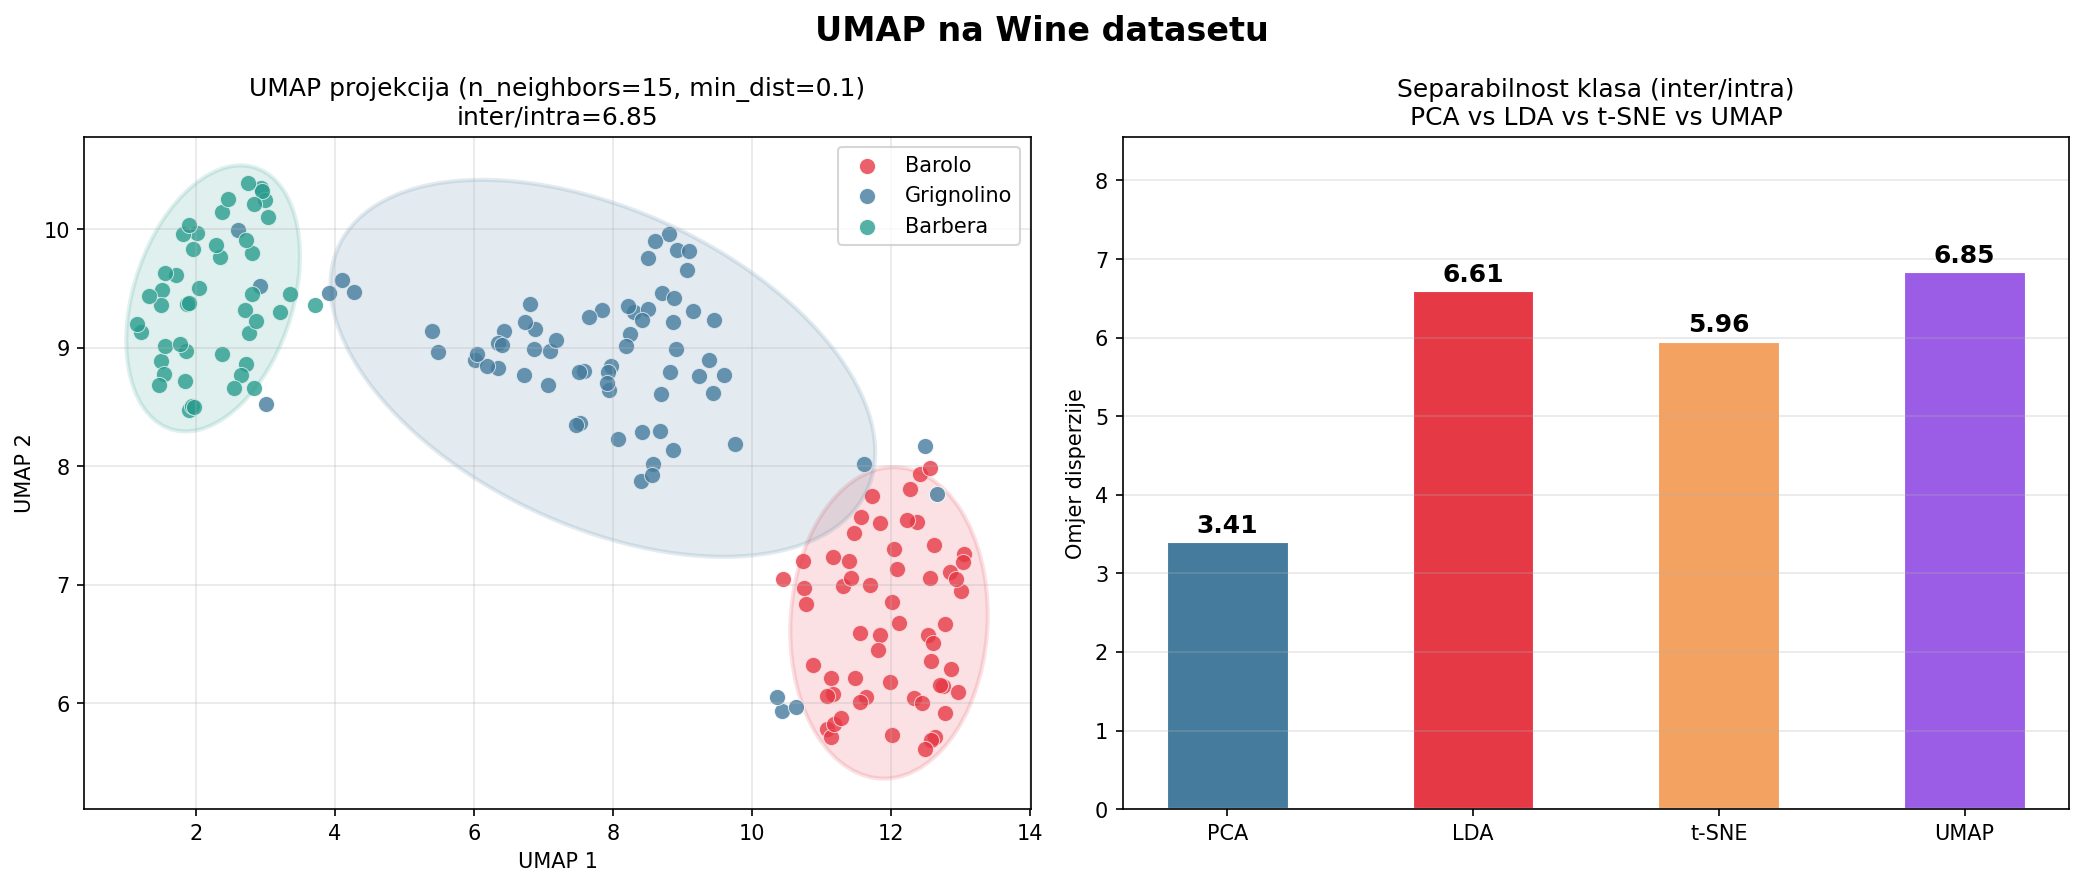
\includegraphics[width=\textwidth]{t02_umap_wine.png}
		\caption{UMAP на Wine скупу: пројекција са елипсама поузданости (лијево) и поређење \textit{inter/intra} односа за сва четири метода (десно).}
		\label{fig:umap_wine}
	\end{figure}
	
	\clearpage
	
	
	\section{Нумерички резултати и поређење метода}
	
	\subsection{Визуелно поређење на истим подацима}
	
	Да бисмо методе директно упоредили, примијенили смо све четири на исти Wine скуп и приказали их једну поред друге (слика \ref{fig:poredenje}). Свака од њих 13-димензионалне податке своди на двије димензије, али то ради на свој начин и са другачијим циљем, па се и резултати међусобно разликују.
	
	PCA тражи правце највеће варијансе, па групе донекле раздваја, али се оне и даље преклапају ($inter/intra = 3{,}41$). LDA користи ознаке класа и циљано раздваја групе, због чега су оне знатно јасније одвојене ($6{,}61$). t-SNE и UMAP, иако не користе ознаке класа, чувају локалну структуру података и дају врло јасно раздвојене групе - t-SNE постиже однос $5{,}96$, а UMAP чак $6{,}85$, што је највећа вриједност међу свим методама. Из ове слике се лијепо види основна разлика: линеарне методе (PCA и LDA) групишу податке праволинијски, док нелинеарне методе (t-SNE и UMAP) могу да ухвате сложеније облике и зато дају компактније и боље одвојене групе.
	
	\begin{figure}[h]
		\centering
		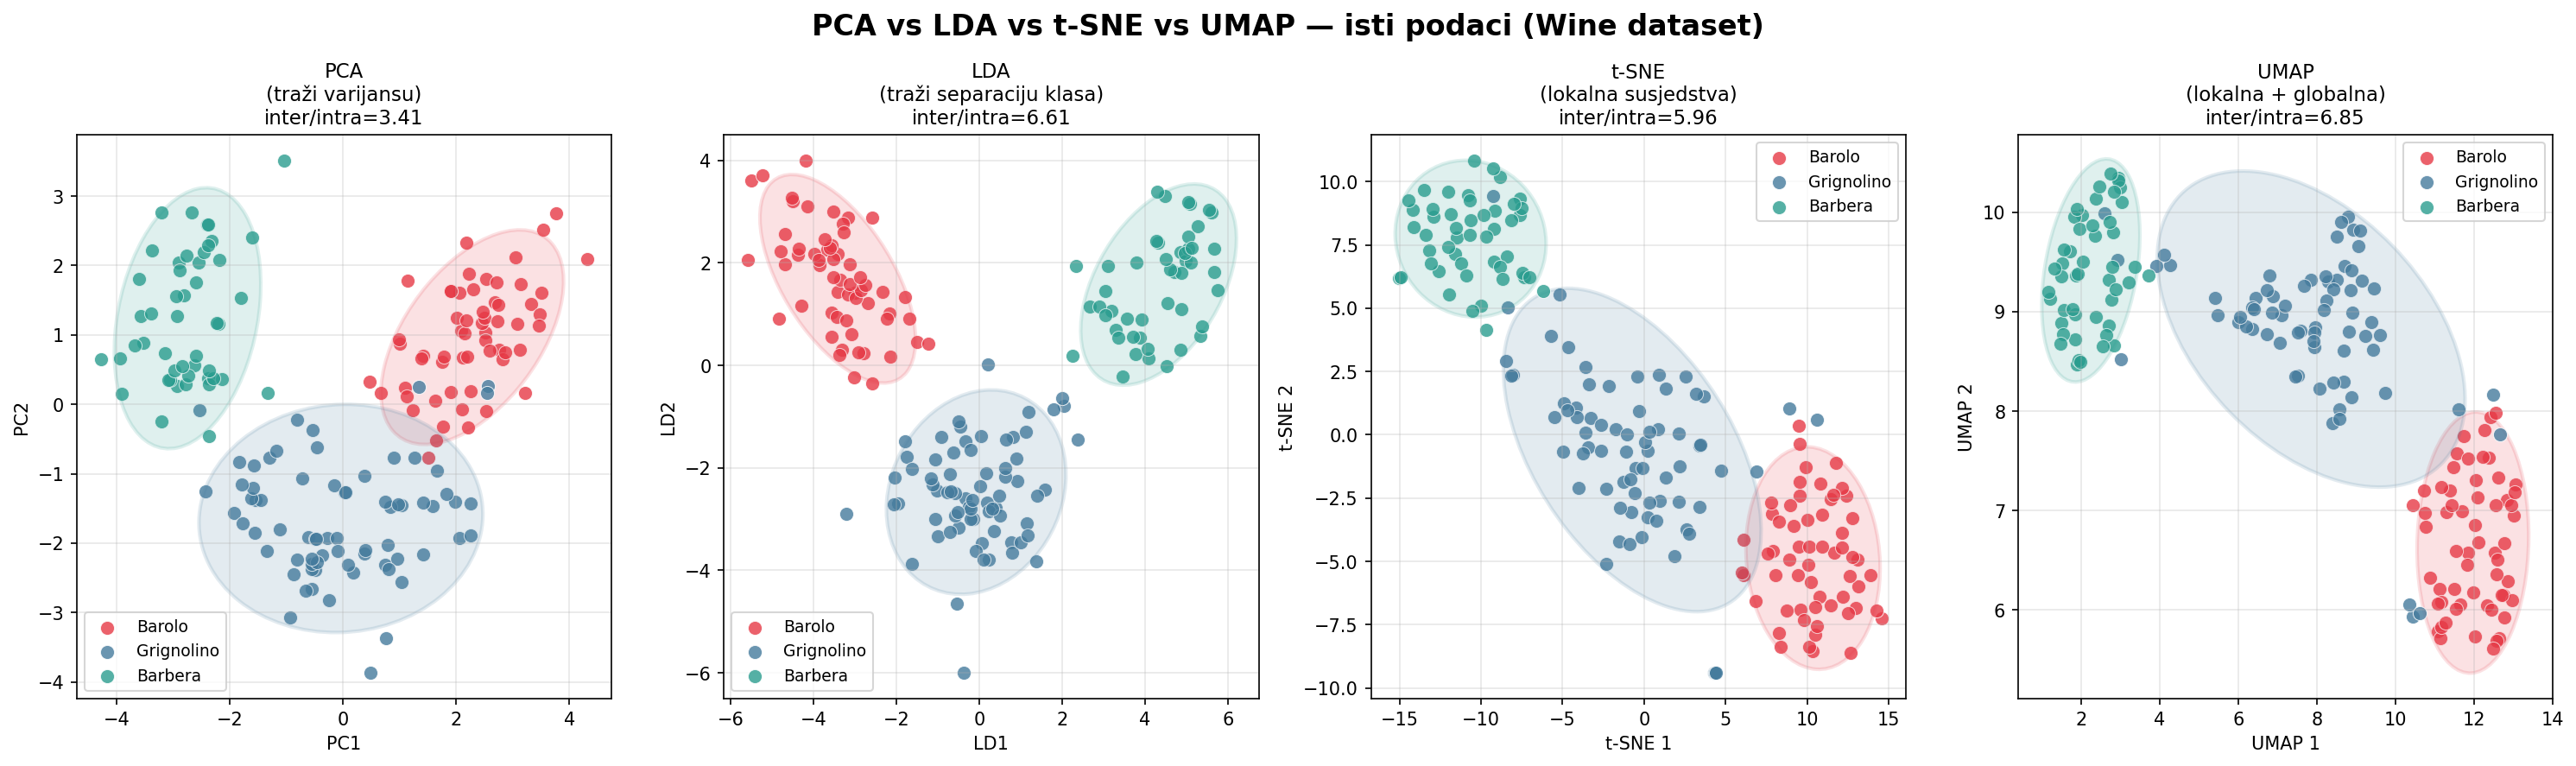
\includegraphics[width=\textwidth]{t04_poredenje.png}
		\caption{PCA, LDA, t-SNE и UMAP - директно поређење на Wine скупу. Сваки панел у наслову исписује \textit{inter/intra} однос.}
		\label{fig:poredenje}
	\end{figure}
	
	
	\subsection{Линеарно наспрам нелинеарног}
	
	Најважнија разлика између линеарних и нелинеарних метода види се када подаци имају нелинеарне границе, односно облике који се не могу раздвојити правом линијом. За провјеру су коришћена два таква примјера: два испреплетена полумјесеца и два концентрична круга (слика \ref{fig:nelinearno}).
	
	На оба примјера линеарне методе (PCA и LDA) заказују. Пошто оне могу само праволинијски да раздвајају податке, не успијевају да прате закривљене облике, па се класе у пројекцији потпуно преклапају. Код концентричних кругова је то посебно изражено - обје класе имају исти центар, па их ни PCA ни LDA не могу раздвојити. Нелинеарне методе (t-SNE и UMAP), с друге стране, гледају локалну структуру података, односно које су тачке једна другој близу, па успијевају да прате и овако сложене облике и јасно раздвоје класе. Овај примјер лијепо показује зашто су нелинеарне методе потребне: оне рјешавају случајеве у којима линеарне методе, чак и надгледана LDA, не могу да помогну.
	
	\begin{figure}[h]
		\centering
		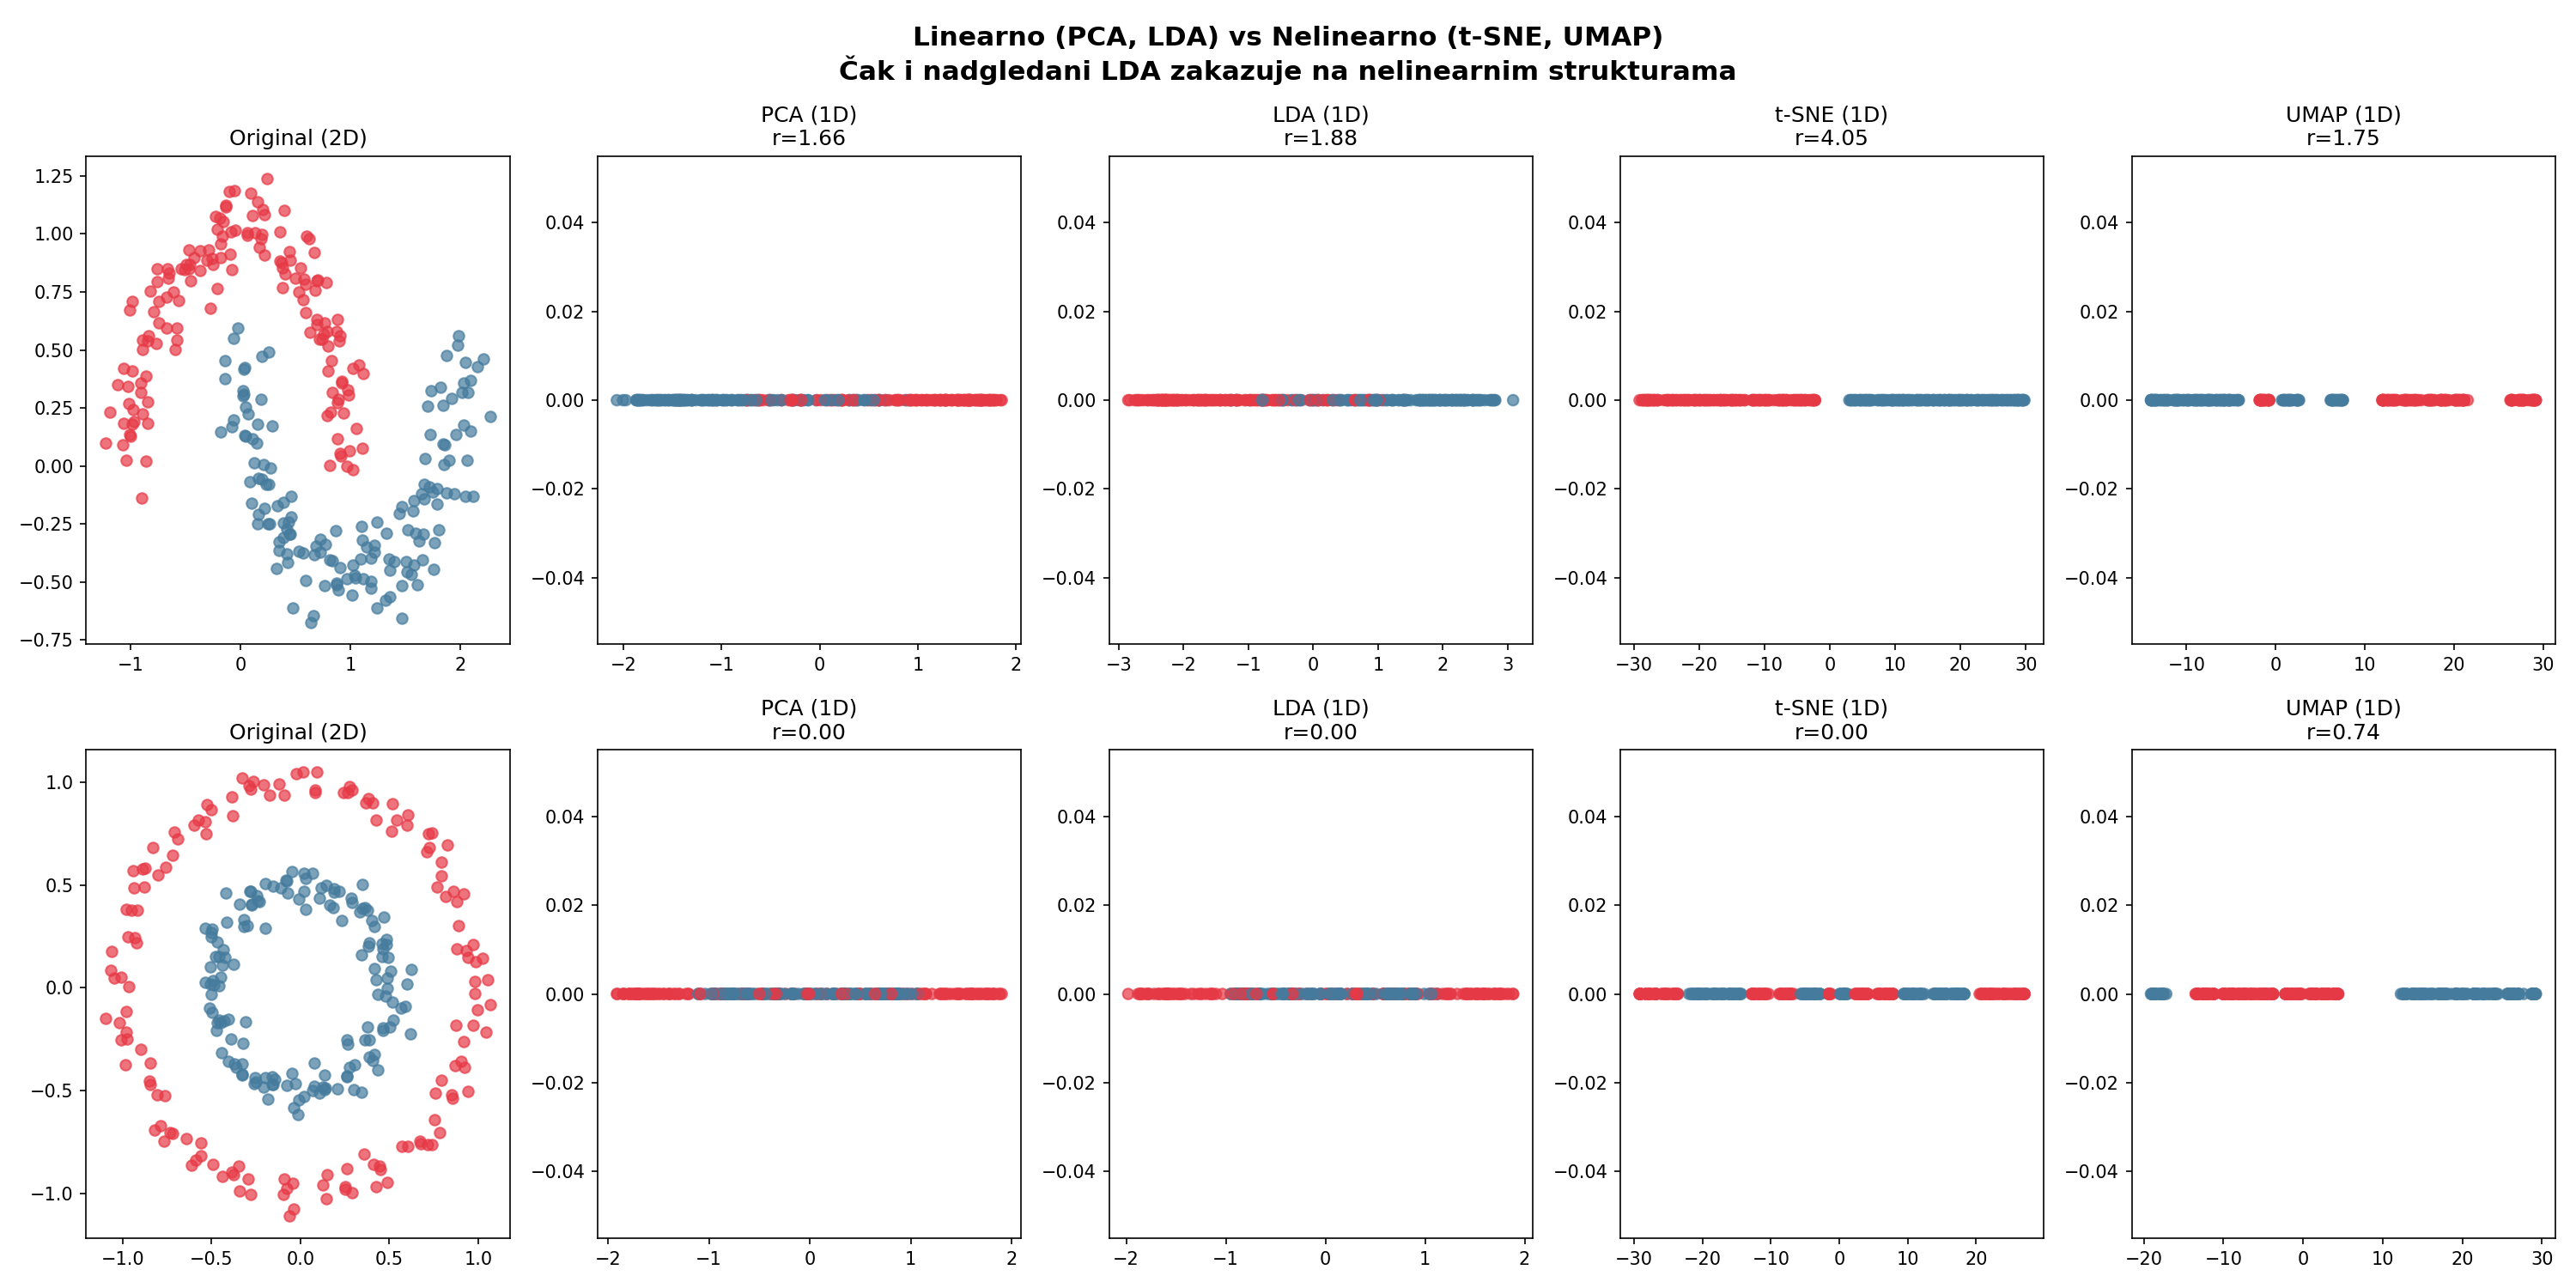
\includegraphics[width=\textwidth]{t05_nelinearne_komplet.png}
		\caption{Линеарне наспрам нелинеарних метода на полумјесецима и концентричним круговима: PCA и LDA заказују (класе се преклапају), док t-SNE и UMAP успјешно раздвајају класе.}
		\label{fig:nelinearno}
	\end{figure}
	
	\clearpage
	
	
	\subsection{Пројекција нових тачака}
	
	Једна од важних практичних разлика између метода јесте да ли могу да пројектују нове, раније невиђене тачке, а да се притом не морају поново покретати над цијелим скупом података (слика \ref{fig:transform}). Ова особина је значајна у пракси, јер се често деси да нови подаци пристигну тек након што је модел већ направљен.
	\begin{itemize}
		\item \textbf{PCA - да.} Модел памти сопствене векторе, па се свака нова тачка једноставно помножи матрицом $\mathbf{W}$ и добије своје координате у новом простору.
		\item \textbf{LDA - да.} Слично као PCA, модел памти дискриминанте, па се нова тачка пројектује истом матрицом, без поновног рачунања.
		\item \textbf{t-SNE - не.} t-SNE нема ту могућност. За сваку нову тачку алгоритам се мора поново покренути над свим подацима, укључујући и старе и нове тачке.
		\item \textbf{UMAP - да.} UMAP памти научени модел, па нове тачке може да пресликава директно, без поновног учења.
	\end{itemize}
	
	Са слике \ref{fig:transform} се види да PCA, LDA и UMAP успјешно смјештају нове тачке (означене звездицама) на очекивана мјеста, међу тачке одговарајућих класа. Код t-SNE то није могуће - нове тачке се не могу додати без поновног покретања алгоритма над цијелим скупом. Управо због ове особине су PCA, LDA и UMAP погоднији за практичне примјене у којима подаци стално пристижу.
	
	\begin{figure}[h]
		\centering
		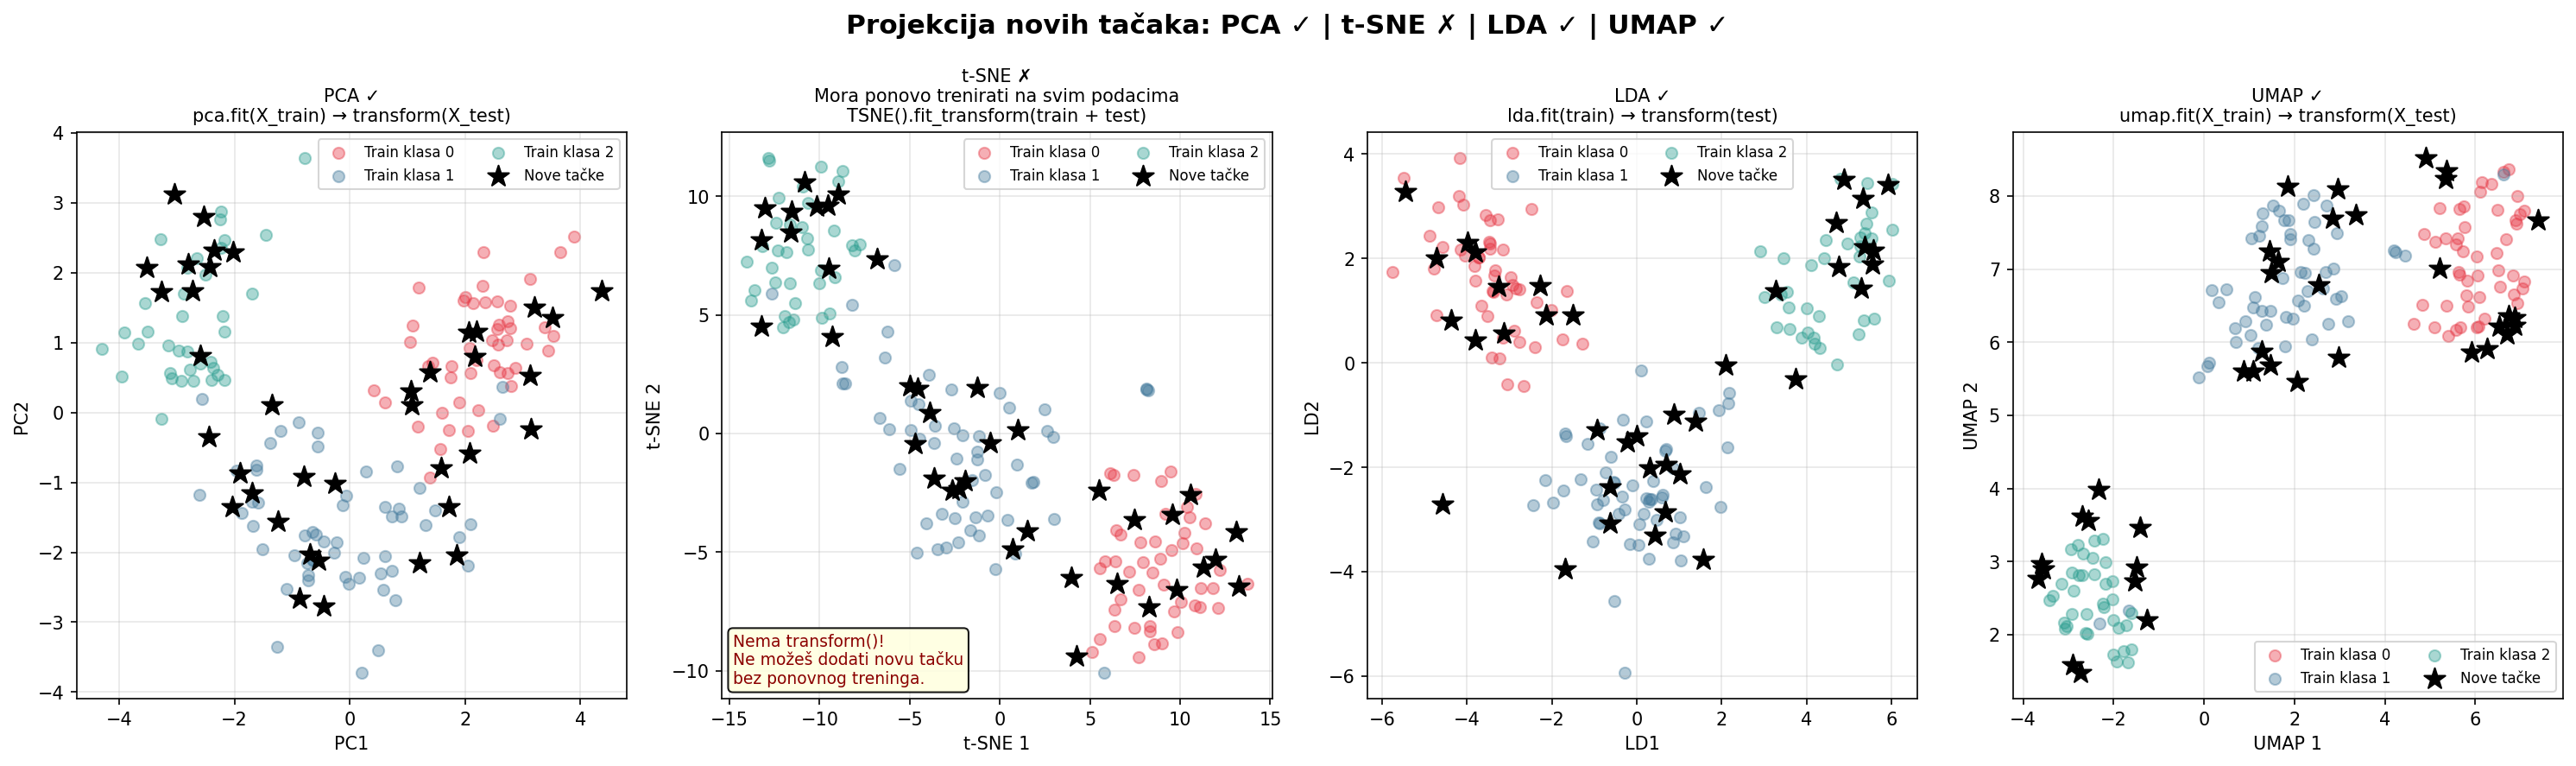
\includegraphics[width=\textwidth]{t08_transform.png}
		\caption{Пројекција нових тачака (звездице): PCA~$\checkmark$, LDA~$\checkmark$, t-SNE~$\times$, UMAP~$\checkmark$. Тренинг подаци приказани су у тамнијој нијанси.}
		\label{fig:transform}
	\end{figure}
	
	
	\subsection{Осјетљивост на одступање}
	
	Још једна разлика између PCA и LDA јесте то колико су осјетљиве на одстуопања, односно на аутлајере - тачке које се налазе далеко од свих осталих. PCA је на њих осјетљива зато што тражи правце највеће варијансе. Једна једина екстремна тачка може знатно да ,,повуче'' главне компоненте у свом смјеру и тако заротира цео координатни систем, чиме се губи сигнал који раздваја класе. LDA је у томе робуснија, јер се ослања на расипање унутар класа које се рачуна из свих тачака заједно, па једна тачка тешко може пресудно да утиче на резултат (слика \ref{fig:outlier}).
	
	На слици \ref{fig:outlier} приказана су оба случаја. У горњем реду, без тачака које одступају, и PCA и LDA лијепо раздвајају двије класе. У доњем реду додата је једна тачка одступања, у тачки $(25, 25)$. Види се да PCA због те једне тачке потпуно губи раздвојеност класа, док LDA остаје стабилна и класе и даље јасно раздваја. Овај примјер показује да PCA треба користити опрезно када подаци садрже одступнице.
	
	\begin{figure}[h]
		\centering
		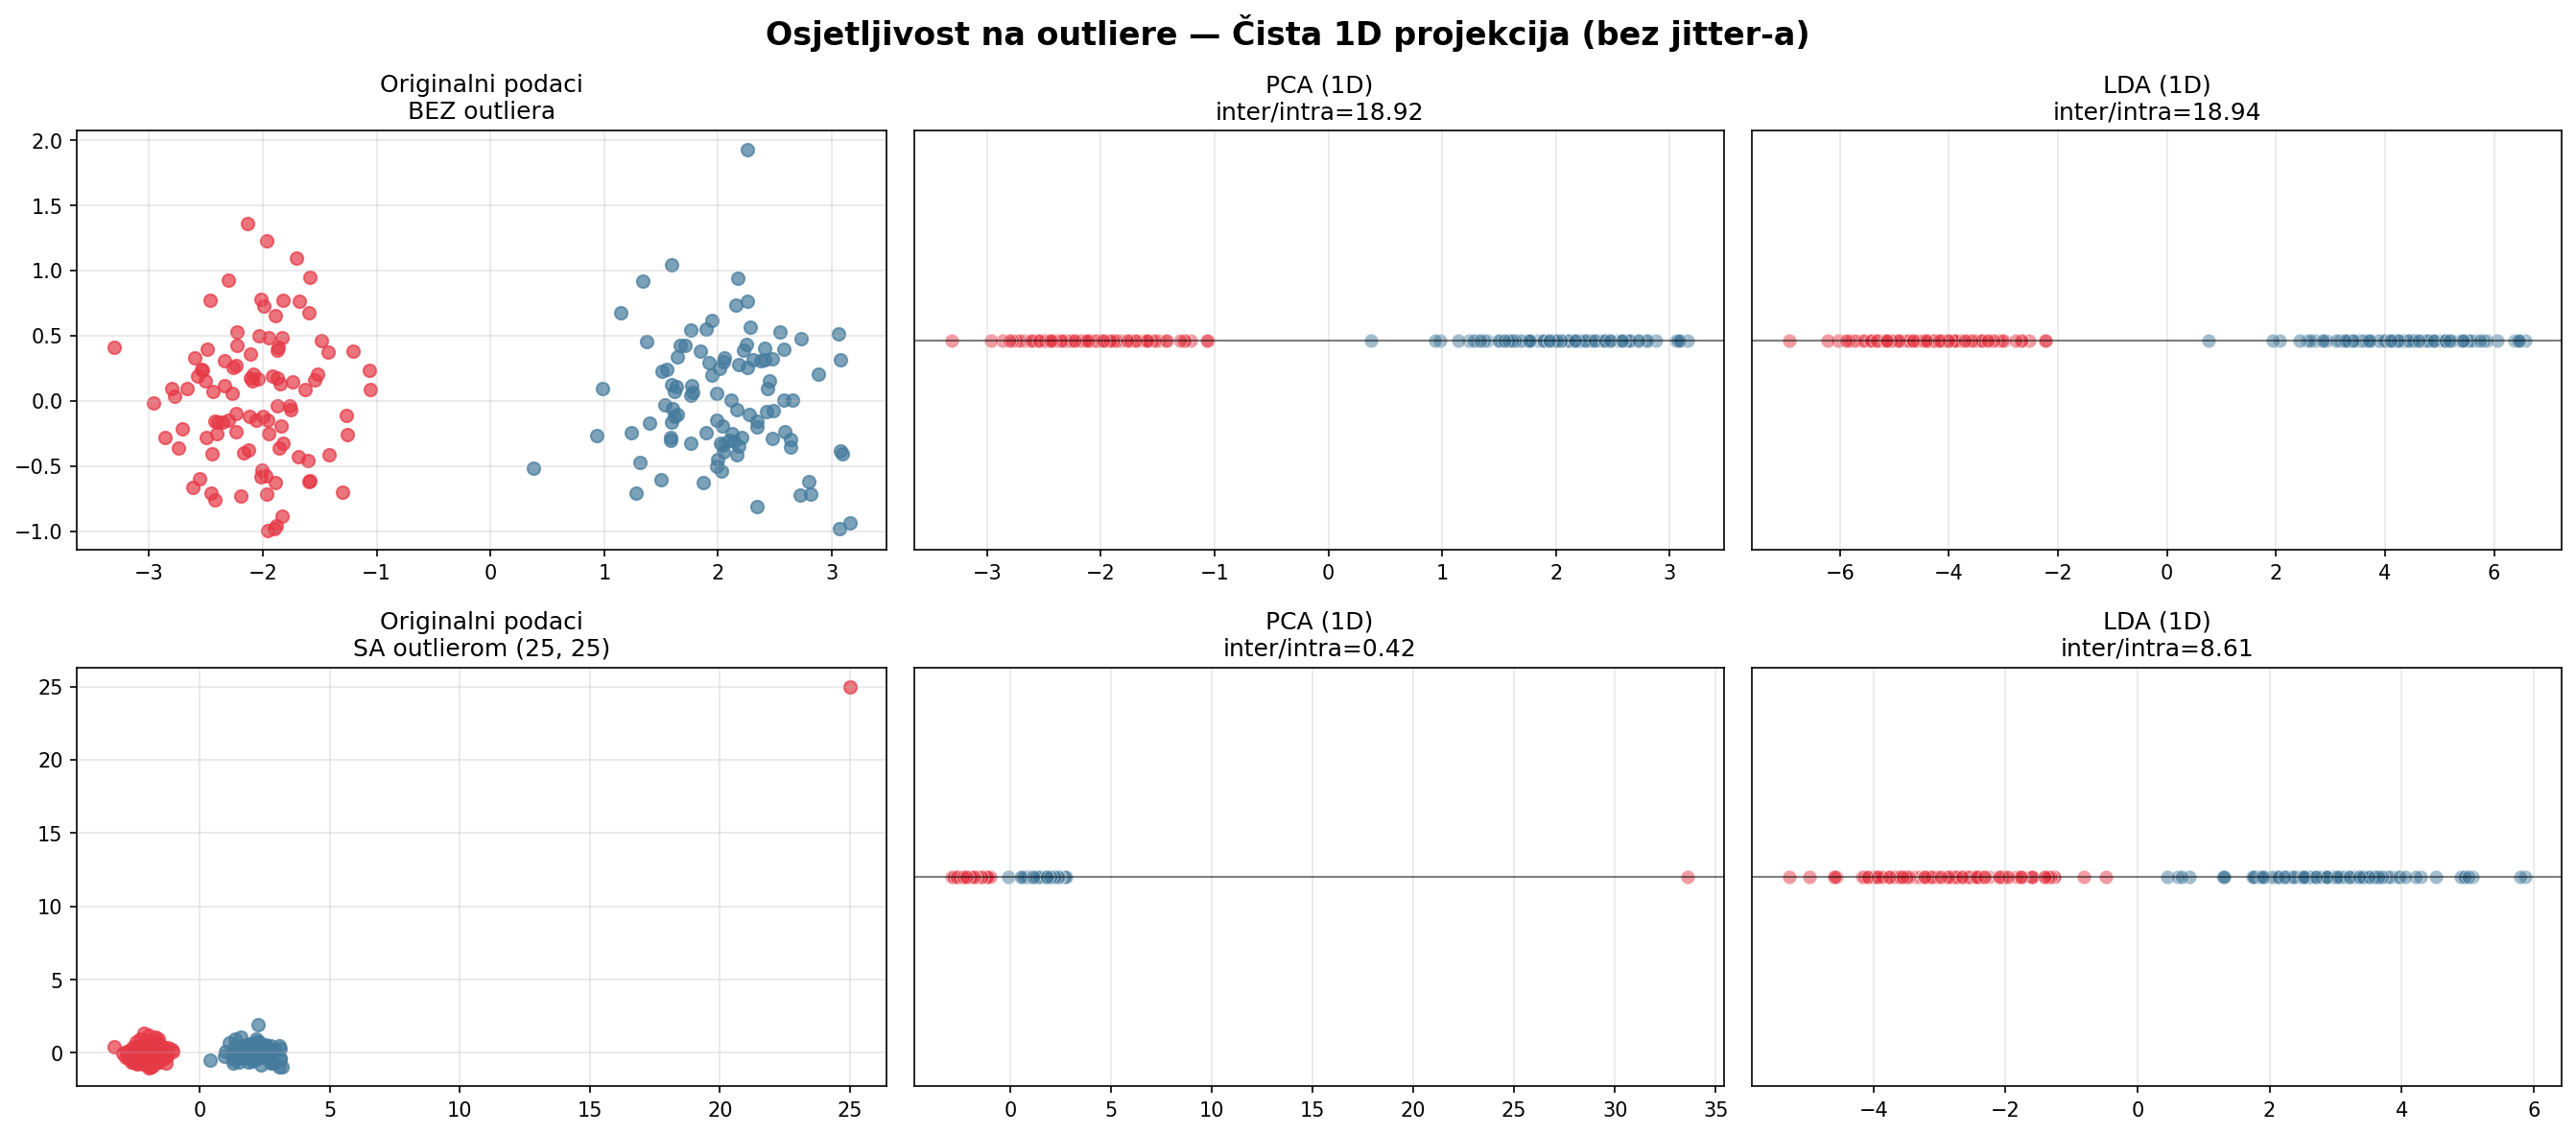
\includegraphics[width=\textwidth]{08_outlier_1D.png}
		\caption{Осјетљивост - PCA наспрам LDA (1Д пројекција).}
		\label{fig:outlier}
	\end{figure}
	
	\clearpage
	
	
	\subsection{Упоредни преглед метода}
	
	У табели \ref{tab:poredenje} дат је збирни преглед свих анализираних метода са њиховим кључним особинама.
	
	\begin{table}[h]
		\centering
		\begin{adjustbox}{center}
			\begin{tabular}{|p{3.5cm}|p{2.3cm}|p{2.3cm}|p{2.3cm}|p{2.3cm}|}
				\hline
				\textbf{Особина} & \textbf{PCA} & \textbf{LDA} & \textbf{t-SNE} & \textbf{UMAP} \\
				\hline
				Тип & Линеарна & Линеарна & Нелинеарна & Нелинеарна \\
				\hline
				Надзор & Ненадгледана & Надгледана & Ненадгледана & Ненадгледана \\
				\hline
				Циљ & Макс. варијанса & Макс. сепарација & Лок. сусједства & Топологија \\
				\hline
				transform() & Да & Да & Не & Да \\
				\hline
				Брзина  & $O(nd^2)$ & $O(nd^2)$ & $O(n^2)$ & $O(n\log n)$ \\
				\hline
				Интерпретабилност & Висока & Висока & Ниска & Ниска \\
				\hline
				Чување глобалне структуре & Да & Да & Дјелимично & Боља \\
				\hline
				Нелинеарне границе & Не & Не & Да & Да \\
				\hline
				Осјет. на параметре & Ниска & Ниска & Висока & Умјерена \\
				\hline
			\end{tabular}
		\end{adjustbox}
		\caption{Поређење свих анализираних метода}
		\label{tab:poredenje}
	\end{table}
	
	
	\subsection{Када користити коју методу?}
	
	На основу свега претходног, може се дати неколико практичних препорука о томе коју методу изабрати у зависности од задатка:
	\begin{itemize}
		\item \textbf{Када је важна интерпретабилност}, односно када треба знати шта нека компонента заправо мјери, најбоља је PCA у комбинацији са \textit{loadings} топлотном мапом, јер она јасно показује које карактеристике доприносе којој компоненти.
		\item \textbf{Када је у питању класификација са унапријед познатим класама}, погодна је LDA као припрема података, будући да боље раздваја класе и тиме побољшава рад класификатора као што су $k$-NN и SVM.
		\item \textbf{Када је циљ визуелно истраживање и откривање група у подацима}, најбоље је користити t-SNE или UMAP, јер јасно приказују групе чак и када су подаци сложени.
		\item \textbf{Када је потребно пројектовати нове тачке}, бирају се PCA, LDA или UMAP, док t-SNE овдје није погодан јер за сваку нову тачку захтијева поновно покретање.
		\item \textbf{Када се ради са великим скуповима података} (преко $50\,000$ узорака), боље је користити PCA или UMAP, пошто је t-SNE у том случају превише спор.
		\item \textbf{Када класе имају нелинеарне границе}, потребне су t-SNE или UMAP, будући да их PCA и LDA не могу раздвојити.
	\end{itemize}
	
	\newpage
	
	
	\section{Закључак}
	
	Смањење димензионалности је једна од основних техника у машинском учењу, која омогућава лакши и ефикаснији рад са подацима високе димензионалности. У овом раду детаљно су описане и упоређене четири методе - PCA, LDA, t-SNE и UMAP - уз нумеричке резултате подробијене на Wine скупу података.
	
	PCA се показала као поуздан избор за линеарну редукцију без надзора. Брза је, детерминистичка, лако се тумачи и подржава пројекцију нових тачака. Због тога је погодна као почетни корак за припрему података, у коме се уклања шум и смањује број димензија прије примјене класификатора. Њено главно ограничење је претпоставка линеарности и осјетљивост на одступнице.
	
	LDA даје најбоље резултате када су ознаке класа познате и када је циљ класификација. Пошто користи информацију о класама, LDA постиже знатно бољу раздвојеност класа од PCA - на Wine скупу чак око 14 пута бољи \textit{inter/intra} однос. Њена ограничења су то што може дати највише $C-1$ дискриминанти и што претпоставља линеарне границе између класа.
	
	t-SNE и UMAP су се показали као моћни алати за визуализацију, посебно када подаци имају нелинеарну структуру. Они успијевају да раздвоје класе које PCA и LDA не могу. Ипак, долазе уз важна упозорења: осе немају физичко значење, резултати зависе од избора хиперпараметара и нису поуздани за мјерење удаљености међу групама. Главна практична разлика међу њима је та што UMAP може да пројектује нове тачке без поновног покретања, док t-SNE то не омогућава, због чега је UMAP погоднији за практичну примјену.
	
	На основу свега изложеног, најбоље рјешење у пракси често је комбиновање метода: PCA се користи за почетну редукцију и уклањање шума, LDA за побољшање раздвојености класа при класификацији, а t-SNE или UMAP за визуализацију и истраживање структуре података. На тај начин се искориштавају предности сваке методе, а умањују њихова појединачна ограничења.
	
	
	\pagebreak
	\begin{thebibliography}{10}

		\bibitem{bishop2006}
		C. M. Bishop, \textit{,,Pattern Recognition and Machine Learning''}, Springer, New York, 2006.

		\bibitem{shlens2014}
		J. Shlens, \textit{,,A Tutorial on Principal Component Analysis''}, arXiv:1404.1100, 2014.

		\bibitem{maaten2008}
		L. van der Maaten and G. Hinton, \textit{,,Visualizing data using t-SNE''}, Journal of Machine Learning Research, vol. 9, pp. 2579--2605, 2008.

		\bibitem{mcinnes2018}
		L. McInnes, J. Healy, and J. Melville, \textit{,,UMAP: Uniform Manifold Approximation and Projection for Dimension Reduction''}, arXiv:1802.03426, 2018.

		\bibitem{coenen2019}
		A. Coenen and A. Pearce, \textit{,,Understanding UMAP''}, Google PAIR Research, 2019. Доступно на: \url{https://pair-code.github.io/understanding-umap/} [Приступљено: 11. јул 2026.].

		\bibitem{matf_pca}
		Математички факултет Универзитета у Београду, \textit{,,Анализа главних компоненти''}. Доступно на: \url{http://old.matf.bg.ac.rs/p/files/69-pca.html} [Приступљено: 11. јул 2026.].

		\bibitem{wine_dataset}
		UCI Machine Learning Repository, \textit{,,Wine Data Set''}, 1991. Доступно на: \url{https://archive.ics.uci.edu/dataset/107/wine} [Приступљено: 11. јул 2026.].

	\end{thebibliography}
	
\end{document}